% ==========================================
% StratosEvent - TCS iON Industry Project Report
% Comprehensive Final Report (60-70 Pages)
% Candidate: Aswini R
% Institute: ICT Academy of Kerala, Thiruvananthapuram
% Track: Web Technology - Full Stack Development
% ==========================================

\documentclass[11pt,a4paper]{report}

\usepackage[T1]{fontenc}
\usepackage[utf8]{inputenc}
\usepackage{helvet}
\usepackage{array}
\usepackage{hyperref}
\usepackage{float}
\usepackage{ragged2e}
\usepackage{tikz}
\usetikzlibrary{shapes.geometric, arrows.meta, positioning, fit, backgrounds, calc}
\usepackage{xcolor}
\usepackage{titlesec}
\usepackage{listings}
\renewcommand{\familydefault}{\sfdefault}

\usepackage[
  a4paper,
  left=1.0in,
  right=1.0in,
  top=1.0in,
  bottom=1.0in,
  headheight=24pt,
  headsep=14pt,
  footskip=36pt
]{geometry}

\usepackage[table]{xcolor}
\usepackage{tabularx}
\usepackage{enumitem}
\usepackage{fancyhdr}
\usepackage{microtype}
\usepackage{anyfontsize}
\usepackage{graphicx}
\usepackage{setspace}
\usepackage{caption}
\usepackage{subcaption}

% 1.22 Line Spacing for Professional Academic Presentation
\setstretch{1.22}

% Official TCS iON Styling Colors
\definecolor{TCSBlue}{HTML}{2E75B6}
\definecolor{TitleBlue}{HTML}{1F4E79}
\definecolor{HeaderGray}{HTML}{555555}
\definecolor{LabelBlue}{HTML}{D9EAF7}
\definecolor{RowGray}{HTML}{F9FBFD}
\definecolor{GridGray}{HTML}{CCCCCC}
\definecolor{CodeBg}{HTML}{F4F6F9}
\definecolor{AccentRed}{HTML}{D32F2F}
\definecolor{SuccessGreen}{HTML}{2E7D32}

\hypersetup{
    colorlinks=true,
    linkcolor=TitleBlue,
    filecolor=magenta,      
    urlcolor=TCSBlue,
    citecolor=TCSBlue,
    pdftitle={StratosEvent: Enterprise Event Management and Dynamic Registration Platform},
    pdfauthor={Aswini R},
    pdfsubject={TCS iON Industry Project Report},
    pdfpagemode=UseBookmarks,
}

% CHAPTER AND SECTION FORMATTING
\titleformat{\chapter}[display]
  {\normalfont\huge\bfseries\color{TitleBlue}}
  {\filleft\Large\sffamily\color{TCSBlue} CHAPTER \thechapter}
  {1ex}
  {\titlerule[1.5pt]\vspace{1.5ex}\filright}
  [\vspace{1ex}\titlerule]

\titlespacing*{\chapter}{0pt}{10pt}{25pt}
\titlespacing*{\section}{0pt}{18pt}{8pt}
\titlespacing*{\subsection}{0pt}{14pt}{6pt}

\titleformat{\section}
  {\normalfont\Large\bfseries\color{TitleBlue}}{\thesection}{1em}{}

\titleformat{\subsection}
  {\normalfont\large\bfseries\color{TCSBlue}}{\thesubsection}{1em}{}

% HEADER AND FOOTER
\pagestyle{fancy}
\fancyhf{}

\fancyhead[L]{%
  \fontsize{9}{11}\selectfont
  \color{HeaderGray}\sffamily
  StratosEvent: Scalable Event Management Platform
}

\fancyhead[R]{%
  \fontsize{9}{11}\selectfont
  \color{HeaderGray}\sffamily
  TCS iON Industry Project
}

\fancyfoot[L]{%
  \fontsize{9}{11}\selectfont
  \color{HeaderGray}\sffamily
  ICT Academy of Kerala
}

\fancyfoot[C]{%
  \fontsize{9}{11}\selectfont
  \color{HeaderGray}\sffamily
  Aswini R
}

\fancyfoot[R]{%
  \fontsize{9}{11}\selectfont
  \color{HeaderGray}\sffamily
  Page \thepage
}

\renewcommand{\headrulewidth}{0.5pt}
\renewcommand{\footrulewidth}{0.5pt}

\renewcommand{\headrule}{%
  \hbox to\headwidth{\color{TCSBlue}%
    \leaders\hrule height \headrulewidth\hfill}
}

\renewcommand{\footrule}{%
  \hbox to\headwidth{\color{TCSBlue}%
    \leaders\hrule height \footrulewidth\hfill}
}

\setlength{\headwidth}{\textwidth}

% Plain page style for chapter beginnings
\fancypagestyle{plain}{%
  \fancyhf{}
  \fancyfoot[C]{\fontsize{9}{11}\selectfont\color{HeaderGray}\sffamily Page \thepage}
  \renewcommand{\headrulewidth}{0pt}
  \renewcommand{\footrulewidth}{0.5pt}
  \renewcommand{\footrule}{%
    \hbox to\headwidth{\color{TCSBlue}\leaders\hrule height \footrulewidth\hfill}
  }
}

% Code Listing Configuration
\lstset{
  basicstyle=\fontsize{8.5}{11}\ttfamily,
  backgroundcolor=\color{CodeBg},
  frame=single,
  rulecolor=\color{GridGray},
  breaklines=true,
  breakatwhitespace=true,
  tabsize=2,
  showstringspaces=false,
  keywordstyle=\color{TCSBlue}\bfseries,
  commentstyle=\color{HeaderGray}\itshape,
  stringstyle=\color{AccentRed}
}



\begin{document}

% ==========================================
% COVER PAGE
% ==========================================
\begin{titlepage}
\thispagestyle{empty}
\begin{center}

  \vspace*{0.4in}

  {\color{TitleBlue}\bfseries
   \fontsize{28}{34}\selectfont
   StratosEvent\par}

  \vspace{0.08in}

  {\color{TitleBlue}\bfseries
   \fontsize{18}{24}\selectfont
   Scalable Event Management, Dynamic Registration\\
   \& Real-Time Attendance Platform\par}

  \vspace{0.25in}

  {\color{TCSBlue}\bfseries
   \fontsize{14}{18}\selectfont
   INDUSTRY PROJECT REPORT\par}

  \vspace{0.15in}

  {\fontsize{11}{16}\selectfont
    A Project Report submitted in partial fulfilment of the requirements\\
    for the award of the Certificate of Internship in the\\
    \textbf{TCS iON Industry Project Programme}\\
    in\\
    \textbf{Web Technology --- Full Stack Development}\\
  }

  \vspace{0.35in}

  % CANDIDATE METADATA TABLE
  \begingroup
  \fontsize{10}{13}\selectfont
  \renewcommand{\arraystretch}{1.45}
  \setlength{\tabcolsep}{8pt}
  \arrayrulecolor{GridGray}

  \noindent
  \begin{tabularx}{0.92\textwidth}{
    |>{\raggedright\arraybackslash\bfseries}p{0.34\textwidth}
    |>{\raggedright\arraybackslash}X|
  }
  \hline
  \cellcolor{LabelBlue} Industry Project Title &
  StratosEvent: Scalable Event Management, Dynamic Registration \& Real-Time Attendance Platform
  \\\hline
  \cellcolor{LabelBlue} Candidate Name &
  \cellcolor{RowGray}Aswini R
  \\\hline
  \cellcolor{LabelBlue} Name of the Institute &
  ICT Academy of Kerala, Thiruvananthapuram
  \\\hline
  \cellcolor{LabelBlue} Academic Specialization &
  Web Technology / Full Stack Web Development
  \\\hline
  \cellcolor{LabelBlue} Sponsoring Platform &
  \cellcolor{RowGray}TCS iON Digital Learning Hub
  \\\hline
  \cellcolor{LabelBlue} GitHub Repository &
  \href{https://github.com/Aswinirkumar/StratosEvent}{\color{TCSBlue}\url{https://github.com/Aswinirkumar/StratosEvent}}
  \\\hline
  \cellcolor{LabelBlue} Submission Date &
  \cellcolor{RowGray}November 2026
  \\\hline
  \end{tabularx}
  \endgroup

  \vspace{0.35in}

  % ENVIRONMENT & EFFORT TABLE
  \begingroup
  \fontsize{9.5}{12}\selectfont
  \renewcommand{\arraystretch}{1.45}
  \setlength{\tabcolsep}{6pt}
  \arrayrulecolor{GridGray}

  \noindent
  \begin{tabularx}{0.92\textwidth}{
    |>{\raggedright\arraybackslash}p{0.14\textwidth}
    |>{\raggedright\arraybackslash}p{0.14\textwidth}
    |>{\raggedright\arraybackslash}p{0.16\textwidth}
    |>{\raggedright\arraybackslash}p{0.20\textwidth}
    |>{\raggedright\arraybackslash}X|
  }
  \hline
  \rowcolor{TCSBlue}
  \color{white}\bfseries Start Date &
  \color{white}\bfseries End Date &
  \color{white}\bfseries Total Effort &
  \color{white}\bfseries Environment &
  \color{white}\bfseries Core Stack \\\hline
  October 2026 &
  November 2026 &
  Approx. 90 hrs &
  Node.js / Windows \& Linux &
  Node.js, Express, MySQL 8.0, HTML5, Bootstrap 5, Vanilla JS (ES6+) \\\hline
  \end{tabularx}
  \endgroup

\end{center}
\end{titlepage}

% ==========================================
% CANDIDATE DECLARATION
% ==========================================
\newpage
\thispagestyle{plain}

\vspace*{0.3in}

\begin{center}
  {\color{TitleBlue}\bfseries\fontsize{18}{22}\selectfont Candidate Declaration\par}
\end{center}

\vspace{0.3in}

\noindent
I, \textbf{Aswini R}, hereby declare that the Industry Project entitled \textbf{``StratosEvent: Scalable Event Management, Dynamic Registration \& Real-Time Attendance Platform''} submitted in partial fulfilment of the requirements of the \textbf{TCS iON Industry Project Programme} in \textbf{Web Technology --- Full Stack Development}, is an authentic record of original engineering work carried out by me under the academic guidance of faculty coordinators at \textbf{ICT Academy of Kerala, Thiruvananthapuram} and industry mentors affiliated with the TCS iON learning ecosystem.

\vspace{0.2in}
\noindent
I further confirm that:
\begin{enumerate}[leftmargin=1.5em, itemsep=0.8em]
    \item The platform design, software implementation, database schema, security mitigations, and test suites presented in this report have been developed by me as part of this internship.
    \item The matter embodied in this report has not been submitted by me or any other individual for the award of any other degree, diploma, or certification at any other institution or university.
    \item All literature, design patterns, documentation standards, and third-party software libraries referenced during this project have been duly acknowledged and cited in the references section.
    \item The source code repositories, automated unit tests, end-to-end verification scripts, and architectural artifacts reflect real, demonstrable engineering implementations executed locally and validated against MySQL 8.0 relational databases.
\end{enumerate}

\vspace{0.6in}

\noindent
\begin{tabularx}{\textwidth}{lXr}
  \textbf{Place:} Thiruvananthapuram & & \textbf{Aswini R} \\
  \textbf{Date:} November 2026 & & Candidate Signature \\
  & & TCS iON Learner ID / Full Stack Intern
\end{tabularx}

% ==========================================
% CERTIFICATE OF COMPLETION
% ==========================================
\newpage
\thispagestyle{plain}

\vspace*{0.3in}

\begin{center}
  {\color{TitleBlue}\bfseries\fontsize{18}{22}\selectfont Certificate of Academic Mentorship\par}
\end{center}

\vspace{0.3in}

\noindent
This is to certify that the project entitled \textbf{``StratosEvent: Scalable Event Management, Dynamic Registration \& Real-Time Attendance Platform''} is a bonafide record of engineering work completed by \textbf{Aswini R} in partial fulfilment of the requirements of the \textbf{TCS iON Industry Project Programme} in \textbf{Web Technology --- Full Stack Development}.

\vspace{0.2in}
\noindent
The project was undertaken in collaboration with \textbf{ICT Academy of Kerala, Thiruvananthapuram} during the period from \textbf{October 2026 to November 2026}. The candidate demonstrated exceptional technical dedication, software architecture proficiency, and rigorous attention to software engineering principles, completing full-stack frontend design, relational schema engineering, transactional concurrency controls, and comprehensive test suite validation.

\vspace{0.2in}
\noindent
The technical outcomes, architectural designs, security assessments, and empirical test results presented within this report have been thoroughly examined and found to meet the high standards expected of professional industry project deliverables.

\vspace{0.8in}

\noindent
\begin{tabularx}{\textwidth}{p{0.45\textwidth}Xp{0.45\textwidth}}
  \rule{0.42\textwidth}{0.4pt} & & \rule{0.42\textwidth}{0.4pt} \\
  \textbf{Project Coordinator / Mentor} & & \textbf{Head of Technical Training} \\
  ICT Academy of Kerala & & ICT Academy of Kerala \\
  Thiruvananthapuram & & Thiruvananthapuram \\
  \\
  \\
  \rule{0.42\textwidth}{0.4pt} & & \rule{0.42\textwidth}{0.4pt} \\
  \textbf{TCS iON Industry Reviewer} & & \textbf{Institutional Seal} \\
  TCS iON Digital Learning Hub & & ICT Academy of Kerala
\end{tabularx}

% ==========================================
% ACKNOWLEDGEMENTS
% ==========================================
\newpage
\thispagestyle{plain}

\vspace*{0.3in}

\begin{center}
  {\color{TitleBlue}\bfseries\fontsize{18}{22}\selectfont Acknowledgements\par}
\end{center}

\vspace{0.3in}

\noindent
The successful design, engineering, and empirical validation of \textbf{StratosEvent} has been an intellectually rewarding journey, made possible through the generous guidance, mentorship, and encouragement of numerous individuals and organizations.

\vspace{0.18in}
\noindent
First and foremost, I express my profound gratitude to the \textbf{TCS iON Industry Project Programme} for curating a hands-on curriculum that bridges academic principles with practical, production-level software development. The problem statements, architectural case studies, and engineering guidelines provided through the TCS iON Digital Learning Hub established a strong foundation for tackling complex challenges such as high-concurrency transactional locking, defense-in-depth web security, and automated quality assurance.

\vspace{0.18in}
\noindent
I extend my sincere appreciation to the faculty members, technical mentors, and leadership of \textbf{ICT Academy of Kerala, Thiruvananthapuram}. Their consistent technical reviews, critical architectural evaluations, and constructive suggestions pushed me to refine every layer of the system---from optimizing relational database indexes in MySQL to ensuring zero horizontal viewport overflow across modern mobile devices.

\vspace{0.18in}
\noindent
I am particularly indebted to my technical mentors who took the time to review my database transaction designs, challenging me to move beyond naive application-level checks and master pessimistic row-level locking with InnoDB. Their insights into securing REST APIs against privilege escalation (CWE-269) and sanitizing roster exports against spreadsheet formula injection (CWE-1236) transformed this project from a standard academic prototype into a resilient, production-ready enterprise platform.

\vspace{0.18in}
\noindent
Finally, I thank my family, peers, and fellow student developers whose unwavering encouragement, patient usability testing, and thoughtful feedback sustained my momentum throughout the intensive development and testing cycles of this project.

\vspace{0.5in}
\begin{flushright}
  \textbf{Aswini R}\\
  \textit{Candidate, TCS iON Industry Project}\\
  ICT Academy of Kerala, Thiruvananthapuram
\end{flushright}

% ==========================================
% ABSTRACT / EXECUTIVE SUMMARY
% ==========================================
\newpage
\thispagestyle{plain}

\vspace*{0.3in}

\begin{center}
  {\color{TitleBlue}\bfseries\fontsize{18}{22}\selectfont Executive Summary / Abstract\par}
\end{center}

\vspace{0.25in}

\justifying
\noindent
Modern event management in educational institutions, technology organizations, and corporate conferences requires reliable software systems capable of handling rapid attendee registrations while guaranteeing strict seat capacity limits. Traditional approaches---frequently relying on shared spreadsheets, basic online form builders, or expensive monolithic software-as-a-service (SaaS) platforms---suffer from critical operational limitations. These include catastrophic overbooking during traffic surges caused by concurrency race conditions, duplicate ticket registrations, lack of custom ticket tier quotas, broken access control vulnerabilities, manual gatekeeper reconciliation delays, and the risk of formula injection in administrative data exports.

\vspace{0.15in}
\noindent
To resolve these challenges, this project presents \textbf{StratosEvent}, an enterprise-grade, highly responsive web application engineered for scalable event discovery, dynamic registration, and real-time attendance verification. Built upon a robust 3-tier architecture, the platform combines a lightweight, zero-build frontend using semantic HTML5, CSS3 Custom Properties, Vanilla JavaScript (ES6+), and Bootstrap 5.3 with a high-throughput Node.js and Express.js REST API service, backed by a fully normalized MySQL 8.0 relational database running the InnoDB storage engine.

\vspace{0.15in}
\noindent
A central technical innovation of StratosEvent is its transactional concurrency engine. Rather than relying on fragile application-level checks, booking operations execute within isolated database transactions governed by pessimistic row-level locking (\texttt{SELECT ... FOR UPDATE}). This guarantees that concurrent seat reservations are strictly serialized at the database engine level, mathematically eliminating overbooking race conditions even under millisecond-interval traffic spikes. Furthermore, the platform introduces flexible per-event ticket tier quotas, enabling event organizers to allocate and enforce custom seat capacities across General, VIP, Student, and Early Bird tiers with real-time remaining-seat indicators.

\vspace{0.15in}
\noindent
Security is implemented using defense-in-depth principles: user authentication utilizes JSON Web Tokens (HS256) and salted bcrypt password hashing, privilege escalation (CWE-269) is eliminated by enforcing server-side role assignment, and administrative CSV exports are systematically neutralized against formula injection (CWE-1236). The system also provides a digital gate-scanner terminal with compound unique constraints preventing duplicate attendee admissions, alongside an executive business intelligence analytics dashboard.

\vspace{0.15in}
\noindent
The platform has been rigorously validated through an automated testing suite comprising 59 unit and integration test cases across 11 test suites and 26 end-to-end integration flows, achieving a \textbf{100\% pass rate} with zero regressions. StratosEvent delivers sub-50ms average API response times, zero horizontal viewport overflow across all mobile, tablet, and desktop screens, and complete institutional data ownership with zero subscription overhead.

\vspace{0.25in}
\noindent
\textbf{Keywords:} Event Management, Concurrency Control, Pessimistic Row Locking, InnoDB ACID Transactions, Ticket Tier Quotas, JWT Authentication, Gate Attendance Verification, Full Stack Web Development, Node.js, Express.js, MySQL 8.0.

% ==========================================
% DYNAMIC TABLES OF CONTENTS, FIGURES, TABLES
% ==========================================
\newpage
\thispagestyle{plain}
\tableofcontents

\newpage
\thispagestyle{plain}
\listoffigures

\newpage
\thispagestyle{plain}
\listoftables

\clearpage



% ==========================================
% CHAPTER 1: INTRODUCTION & PROJECT OVERVIEW
% ==========================================
\chapter{Introduction \& Project Overview}

\section{Context and Background}
\justifying
Over the past decade, the rapid expansion of academic symposiums, technical hackathons, professional webinars, and developer conferences has transformed event management into a mission-critical operational workflow for educational institutions and corporate enterprises alike. Coordinating an event involves multifaceted responsibilities: publishing clear schedules, publicizing speaker agendas, managing seat capacities, facilitating frictionless attendee registrations, issuing verifiable admission passes, checking in participants at the venue, and analyzing post-event attendance metrics.

Historically, academic departments and small-to-medium organizations have managed these workflows through ad-hoc, informal mechanisms. Event organizers frequently shared online spreadsheets across committees or created uncoordinated web forms. While these manual methods appear convenient during the planning phase, they consistently break down when an event opens for active registration. In high-demand scenarios---such as a hands-on machine learning workshop with limited computer lab workstations or an executive networking dinner with strict venue fire codes---hundreds of prospective attendees attempt to register simultaneously.

When multiple users submit booking requests within fractions of a second, naive tools and informal databases fail catastrophically. The absence of transactional concurrency control leads to severe overbooking, duplicate registrations, and administrative confusion. Organizers are forced to spend hours manually reconciling conflicting records, issuing embarrassing cancellation notices, or dealing with overcrowded rooms. Furthermore, traditional paper-based check-in rosters at venue entrances cause severe bottlenecks, where attendees wait in long queues while staff cross-reference names on printed sheets.

These widespread operational vulnerabilities highlight the urgent need for a dedicated, unified, and resilient digital event management platform. Modern event software must not only deliver an appealing and intuitive discovery interface for attendees, but must also be anchored by an enterprise-grade backend capable of enforcing mathematical capacity limits, protecting user privacy, and streamlining gatekeeper operations.

\section{Motivation and Problem Statement}
\justifying
The primary motivation behind the development of \textbf{StratosEvent} stems from direct observations of the systemic failures prevalent in conventional event coordination tools. Through a detailed analysis of existing academic and industry event practices, we identified five critical vulnerabilities that severely degrade event operations:

\begin{enumerate}[leftmargin=1.5em, itemsep=0.8em]
    \item \textbf{Transactional Overbooking and Concurrency Race Conditions:} In standard web architectures, checking whether seats are available and subsequently recording a registration are handled as separate, non-atomic database operations. When ten users request the last remaining seat at the exact same millisecond, naive application logic checks the count, observes that one seat remains for each user, and inserts all ten registrations. This race condition leads to severe venue overcapacity, fire-safety compliance breaches, and frustrated attendees.
    \item \textbf{Duplicate Bookings and Phantom Capacity Consumption:} Due to intermittent mobile network connectivity or eager double-clicking by users, registration requests are often dispatched multiple times in rapid succession. In the absence of strict compound unique keys at the database engine level, identical records are created, artificially exhausting seat availability and leaving physical seats empty on event day.
    \item \textbf{Privilege Escalation and Insecure Role Assignment (CWE-269):} Many rapid-development web applications accept user registration payloads containing arbitrary attributes, such as client-supplied role parameters. Without server-side validation and cryptographic verification, malicious participants can easily grant themselves administrative rights, gaining unauthorized control over event configurations and sensitive attendee rosters.
    \item \textbf{Manual Gatekeeper Bottlenecks and Ticket Fraud:} At physical venue entrances, relying on paper rosters or unverified static PDF passes leads to substantial operational friction. Static tickets can be easily duplicated, shared, or forged, allowing unauthorized individuals to enter while staff struggle to maintain an accurate count of admitted attendees.
    \item \textbf{Vulnerable Administrative Data Exports (CWE-1236):} Event organizers routinely export attendee rosters to CSV format for offline processing and reporting. If an attendee registers with a name starting with formula trigger characters (such as \texttt{=}, \texttt{+}, \texttt{-}, or \texttt{@}), opening the unescaped CSV file in standard spreadsheet software can execute malicious macros or exfiltrate data, exposing institutional computers to compromise.
\end{enumerate}

StratosEvent was specifically conceived, architected, and built to eliminate each of these vulnerabilities through rigorous software engineering, modern web standards, and transactional database guarantees.

\section{Project Goals and Core Objectives}
\justifying
The overarching goal of the StratosEvent project is to engineer a production-ready, highly responsive, full-stack web application that unifies event discovery, atomic seat reservation, granular ticket tier allocation, gate admission verification, and executive reporting into a cohesive platform.

To achieve this goal, the project was organized around seven specific, measurable engineering objectives:

\begin{enumerate}[leftmargin=1.5em, itemsep=0.8em]
    \item \textbf{Deliver a Frictionless, Discovery-First User Experience:} Build an accessible, modern frontend interface that allows participants to explore upcoming events effortlessly, apply instant multi-criteria filters across categories (Workshops, Webinars, Conferences, Hackathons, and Seminars), and view live seat availability without cumbersome full-page reloads.
    \item \textbf{Implement Granular Per-Event Ticket Tier Quotas:} Provide event organizers with the ability to allocate explicit seat capacity quotas across distinct ticket tiers---General Admission, VIP Access, Student Discount, and Early Bird---with automatic sum-to-capacity validation and live remaining-seat status indicators (such as \textit{14 left}, \textit{Sold Out}, or \textit{Not Offered}).
    \item \textbf{Guarantee Mathematical Capacity Integrity via ACID Locking:} Implement pessimistic row-level locking using MySQL InnoDB transactions (\texttt{SELECT ... FOR UPDATE}), ensuring that high-concurrency booking rushes are strictly serialized at the database layer and completely preventing overbooking.
    \item \textbf{Establish Defense-in-Depth Authentication and Access Controls:} Architect a stateless authentication subsystem utilizing JSON Web Tokens (HS256) and salted bcrypt password hashing, strictly hardcoding public registrations to participant privileges and eliminating privilege escalation vectors.
    \item \textbf{Support Complete Attendee Lifecycle Moderation:} Provide administrative moderation capabilities across four distinct registration states (\texttt{pending}, \texttt{approved}, \texttt{rejected}, and \texttt{cancelled}), complete with automatic inventory replenishment whenever a confirmed reservation is cancelled.
    \item \textbf{Deploy a Tamper-Resistant Gatekeeper Verification Scanner:} Equip venue check-in staff with a streamlined ticket validation terminal that verifies cryptographically structured ticket codes and records admissions with atomic duplicate check-in prevention.
    \item \textbf{Generate Real-Time Executive Analytics with Sanitized CSV Export:} Deliver an executive intelligence dashboard tracking capacity utilization, attendance conversion ratios, and participant demographics, complemented by an RFC 4180-compliant CSV export engine secured against spreadsheet formula injection.
\end{enumerate}

\section{Project Scope: Included vs. Excluded Boundaries}
\justifying
Establishing clear functional and technical boundaries was critical to ensuring the timely, high-quality delivery of the StratosEvent platform within the internship timeline.

\subsection{Included Capabilities and System Scope}
The StratosEvent project scope encompasses the full software development lifecycle, including requirements engineering, relational database design, REST API implementation, frontend interface development, security hardening, and automated test validation:
\begin{itemize}[leftmargin=1.5em, itemsep=0.4em]
    \item Complete full-stack architecture running Node.js, Express.js, and MySQL 8.0 InnoDB.
    \item Native, zero-build responsive frontend interface utilizing semantic HTML5, CSS3 Custom Properties, Vanilla JavaScript (ES6+), and Bootstrap 5.3 components.
    \item Dynamic event catalog supporting real-time client-side search, category filtering, and live capacity chips.
    \item Flexible ticket tier allocation module supporting General, VIP, Student, and Early Bird quotas with interactive visual management in administrative consoles.
    \item Robust authentication subsystem supporting user registration, secure login, profile inspection, and token verification.
    \item Participant self-service dashboard (``My Tickets \& Passes'') rendering official confirmed booking passes with unique ticket codes and one-click cancellation.
    \item Unified administrator control console providing registration moderation, event creation, live event editing, gate attendance scanning, and business intelligence reporting.
    \item Sanitized CSV roster export module implementing formula neutralization guards.
    \item Exhaustive automated test suite featuring 59 unit and integration tests across 11 test suites and 26 end-to-end operational verification flows.
\end{itemize}

\subsection{Excluded Elements and Future Scope Boundaries}
To maintain focus on core transactional reliability and institutional usability, the following elements were intentionally placed outside the current development scope:
\begin{itemize}[leftmargin=1.5em, itemsep=0.4em]
    \item \textbf{Physical Optical Hardware Integration:} The current system provides a high-efficiency software verification terminal; direct integration with specialized laser turnstile barcode hardware was excluded.
    \item \textbf{Monetary Payment Gateway Processing:} The platform manages seat reservations and capacity quotas; direct financial transactions through credit card processors were deferred to future iterations.
    \item \textbf{Native Mobile App Binaries:} Rather than maintaining separate Objective-C/Swift and Java/Kotlin codebases, the platform was developed using mobile-first responsive web design principles, guaranteeing flawless operation on all standard mobile browsers without horizontal viewport overflow.
\end{itemize}

\section{Report Organization}
\justifying
The remainder of this report is structured systematically to document the engineering methodology, architectural decisions, and empirical results of the StratosEvent platform:
\begin{itemize}[leftmargin=1.5em, itemsep=0.4em]
    \item \textbf{Chapter 2 (Literature Survey \& Comparative Analysis):} Evaluates existing event management approaches, contrasts their capabilities in a detailed matrix, and identifies the core technical gaps addressed by StratosEvent.
    \item \textbf{Chapter 3 (Software Requirements Specification):} Outlines stakeholder personas, detailed functional requirements (FR-01 through FR-12), non-functional requirements, and system feasibility.
    \item \textbf{Chapter 4 (System Architecture \& Database Design):} Details the 3-tier system architecture, transactional workflow flowcharts, 3NF relational database schema, data dictionaries, ER diagram, and REST API endpoint contracts.
    \item \textbf{Chapter 5 (System Implementation \& Engineering Deep Dive):} Explains the practical implementation of stateless JWT authentication, InnoDB row-level locking, per-tier seat quotas, gate verification, and CSV formula sanitization.
    \item \textbf{Chapter 6 (Quality Assurance \& Testing Suite):} Presents the automated testing methodology, detailing the 59 passing unit/integration test cases, 26 end-to-end flows, and concurrency stress testing outcomes.
    \item \textbf{Chapter 7 (Results \& User Interface Walkthrough):} Provides an annotated, figure-by-figure walkthrough of all 13 core user interfaces across attendee and administrator workflows.
    \item \textbf{Chapter 8 (Challenges, Security Audits \& Lessons Learned):} Discusses key engineering hurdles overcome, security vulnerability mitigations, and personal technical reflections.
    \item \textbf{Chapter 9 (Future Enhancements \& Conclusion):} Summarizes project achievements, outlines future development roadmaps, and provides code execution guidelines.
\end{itemize}



% ==========================================
% CHAPTER 2: LITERATURE SURVEY & COMPARATIVE ANALYSIS
% ==========================================
\chapter{Literature Survey \& Comparative Analysis}

\section{Evolution of Event Management Systems}
\justifying
The management of professional and academic events has undergone significant evolution over the past three decades. In the early eras of computing, event coordination was entirely manual, relying on physical bulletin boards, printed paper registration forms, and manual ledger books. Event coordinators spent substantial manual effort transcribing handwritten attendee information into departmental filing cabinets, issuing paper admission receipts, and manually verifying identities at physical entrance doors.

With the widespread advent of personal computing and local area networks in the 1990s, organizations began adopting desktop database software and digital spreadsheet applications such as Microsoft Excel. While this transition eliminated paper filing cabinets and allowed basic digital roster storage, it introduced new coordination problems: multiple organizers frequently maintained conflicting copies of the same spreadsheet on separate desktop workstations, leading to widespread version mismatch and lost updates.

The emergence of cloud computing and collaborative web applications in the late 2000s facilitated the rise of shared online documents (such as Google Sheets) and web form builders (such as Google Forms and Typeform). These platforms enabled decentralized data entry and streamlined participant data collection. However, as event scale and concurrency increased, these general-purpose tools revealed fundamental architectural limitations when applied to high-demand ticketing scenarios. Concurrently, commercial event software-as-a-service (SaaS) providers emerged, offering comprehensive feature sets but imposing high subscription costs, rigid payment workflows, and proprietary data lock-in.

\section{Evaluation of Existing Approaches}
\justifying
To establish a clear technical foundation for StratosEvent, we conducted a rigorous comparative analysis of the three predominant approaches currently utilized across educational institutions and commercial enterprises.

\subsection{Shared Collaborative Spreadsheets (Google Sheets, Microsoft Excel Online)}
Shared spreadsheets remain widely utilized due to their familiarity and zero setup friction. Non-technical staff can rapidly create columns for attendee names, contact details, and payment statuses. However, when evaluated against enterprise software engineering standards, spreadsheets exhibit severe structural deficiencies:
\begin{itemize}[leftmargin=1.5em, itemsep=0.4em]
    \item \textbf{Absence of Concurrency Controls:} Spreadsheets have no concept of transactional row locking or ACID isolation. When multiple coordinators or automated scripts attempt to modify participant statuses or update capacity counters simultaneously, race conditions routinely cause lost updates and record overwrites.
    \item \textbf{Lack of Data Integrity and Referential Constraints:} Spreadsheets do not enforce foreign key relationships or compound uniqueness constraints. Attendees can easily register multiple times with minor typographical variations, distorting capacity planning.
    \item \textbf{Inadequate Security and Access Granularity:} Access control in shared spreadsheets is binary (view or edit permissions across the entire document). Sensitive attendee data---including email addresses and contact numbers---is exposed to all individuals granted access, violating basic data privacy standards.
\end{itemize}

\subsection{Generic Online Form Builders (Google Forms, Typeform, Microsoft Forms)}
Online form builders provide a streamlined public interface for collecting survey and registration data, automatically appending responses to an underlying spreadsheet or database. While effective for simple surveys, form builders are ill-suited for transactional event ticketing:
\begin{itemize}[leftmargin=1.5em, itemsep=0.4em]
    \item \textbf{Passive Data Collection without Atomic Capacity Enforcement:} Form builders collect submissions passively. They lack server-side locking mechanisms to halt registrations the exact instant venue capacity is reached. By the time an organizer notices that 150 responses have been submitted for a 100-seat room, the event is already severely overbooked.
    \item \textbf{No Support for Dynamic Ticket Tier Quotas:} Standard form builders treat all submissions identically. They cannot dynamically allocate or track separate quotas for General, VIP, Student, and Early Bird tiers, nor can they disable individual tiers in real time as specific limits are exhausted.
    \item \textbf{Missing Gatekeeper Verification Workflow:} Form builders offer no built-in mechanism for generating cryptographically verifiable ticket codes, inspecting passes at the venue entrance, or preventing duplicate check-ins.
\end{itemize}

\subsection{Commercial Monolithic SaaS Platforms (Eventbrite, Meetup, Cvent)}
Commercial SaaS platforms represent the most feature-complete solutions in the industry, offering integrated marketing, registration workflows, mobile check-in applications, and payment processing. However, their architecture introduces substantial organizational drawbacks:
\begin{itemize}[leftmargin=1.5em, itemsep=0.4em]
    \item \textbf{Prohibitive Financial Costs and Fee Structures:} Commercial platforms monetize either through substantial monthly software subscriptions or by charging high percentage-based fees on every issued ticket. For educational institutions, non-profit academic symposiums, and student-run hackathons operating on tight budgets, these recurring fees are prohibitive.
    \item \textbf{Loss of Institutional Data Sovereignty:} Storing student and corporate attendee data on third-party commercial cloud servers introduces legal and privacy compliance concerns (such as GDPR and local data protection regulations). Institutions lose direct control over how attendee information is processed and retained.
    \item \textbf{Rigid Workflow Constraints and Heavy Client Overhead:} Commercial platforms enforce standardized registration forms and complex ticketing workflows that cannot be tailored to departmental policies. Furthermore, their web interfaces rely on heavy client-side JavaScript bundles exceeding multiple megabytes, resulting in sluggish load times on lower-powered devices and slow mobile connections.
\end{itemize}

\section{Comparative Analysis Matrix}
\justifying
Table~\ref{tab:comparative_analysis} synthesizes this evaluation, contrasting the capabilities of spreadsheets, form builders, commercial SaaS solutions, and StratosEvent across ten critical operational and engineering criteria.

\begin{table}[H]
\centering
\fontsize{8.5}{11}\selectfont
\renewcommand{\arraystretch}{1.35}
\setlength{\tabcolsep}{4pt}
\arrayrulecolor{GridGray}
\caption{Comprehensive Comparative Evaluation of Event Management Paradigms}
\label{tab:comparative_analysis}
\begin{tabularx}{\textwidth}{|p{0.24\textwidth}|X|X|X|X|}
\hline
\rowcolor{TCSBlue}
\color{white}\bfseries Feature / Metric & 
\color{white}\bfseries Spreadsheets & 
\color{white}\bfseries Form Builders & 
\color{white}\bfseries Commercial SaaS & 
\color{white}\bfseries StratosEvent \\\hline

\textbf{Overbooking Guard} & None (Race Prone) & Naive Post-Check & Vendor Managed & \textbf{ACID Pessimistic Lock} \\\hline
\textbf{Ticket Tier Quotas} & Manual Formulas & Unsupported & Supported (Paid) & \textbf{Native Dynamic Quotas} \\\hline
\textbf{Concurrency Safety} & Lost Updates & Double Submissions & Proprietary & \textbf{InnoDB Serialized Locks} \\\hline
\textbf{Access Control} & Document-level & Shared Links & Proprietary RBAC & \textbf{JWT Stateless Guard} \\\hline
\textbf{Gate Check-In} & Paper Cross-Off & External Add-on & Native Mobile App & \textbf{Integrated Web Terminal} \\\hline
\textbf{Duplicate Check-In} & Vulnerable & Unsupported & Supported & \textbf{Enforced by Unique Key} \\\hline
\textbf{Data Ownership} & Dispersed & Third-Party Cloud & Proprietary Cloud & \textbf{100\% Self-Hosted MySQL} \\\hline
\textbf{CSV Injection Guard} & None & None & Inconsistent & \textbf{Sanitized (CWE-1236)} \\\hline
\textbf{Client Footprint} & Heavy Web App & Light Survey Form & Heavy Script Bundle & \textbf{Zero-Build Native ES6} \\\hline
\textbf{Financial Cost} & Subscription & Freemium Limits & Expensive Fees & \textbf{Zero Subscription (Open)} \\\hline
\end{tabularx}
\end{table}

\section{Identified Research Gaps and the StratosEvent Paradigm}
\justifying
Our literature survey and practical evaluations revealed a clear void in modern web tooling: \textbf{the absence of an open, lightweight, self-hosted event platform that pairs consumer-grade event discovery with rigorous, database-level transactional concurrency control.}

Most existing custom event scripts developed in academia or small enterprises suffer from architectural shortcuts. Developers frequently perform seat availability checks in application memory or through standard non-locking database queries (such as \texttt{SELECT COUNT(*) FROM registrations}). Under normal testing with one or two simulated users, this approach appears to function correctly. However, in real-world high-demand scenarios where dozens of requests arrive within the same millisecond, non-locking reads permit multiple requests to observe available seats simultaneously, resulting in catastrophic overbooking.

StratosEvent directly addresses this gap by implementing an enterprise architectural paradigm centered around three core tenets:
\begin{enumerate}[leftmargin=1.5em, itemsep=0.6em]
    \item \textbf{Database-Level Transactional Authority:} Rather than trusting application memory or optimistic counters, the database engine is treated as the single authoritative source of truth. Every booking operation is enclosed in an atomic transaction governed by pessimistic row-level locking.
    \item \textbf{Granular Quota Customization Without Relational Bloat:} By embedding dedicated tier quota columns directly within the core event entity, StratosEvent delivers per-tier seat allocation without requiring complex multi-table joins during high-traffic catalog queries.
    \item \textbf{Zero-Build High-Performance Presentation:} By utilizing native modern JavaScript (ES6+), semantic HTML5, and CSS Custom Properties, the platform delivers instantaneous page transitions and responsive user feedback without the multi-megabyte bundle overhead or build-step fragility of modern single-page application frameworks.
\end{enumerate}



% ==========================================
% CHAPTER 3: SOFTWARE REQUIREMENTS SPECIFICATION
% ==========================================
\chapter{Software Requirements Specification (SRS)}

\section{Stakeholder Analysis and User Personas}
\justifying
A successful event platform must accommodate diverse user groups with distinct technical proficiencies, objectives, and operational responsibilities. StratosEvent was engineered around four clearly defined stakeholder personas:

\begin{enumerate}[leftmargin=1.5em, itemsep=0.8em]
    \item \textbf{Participant / Attendee (Public User):} Prospective attendees range from university students seeking skill-building workshops to industry professionals attending technical conferences. Their primary goals are rapid event discovery, reviewing detailed event agendas and prerequisites, checking remaining seat availability across ticket tiers, securing a confirmed reservation with minimal friction, and accessing their verified digital ticket pass from mobile devices.
    \item \textbf{Event Coordinator / Organizer:} Faculty coordinators, departmental heads, or committee organizers responsible for scheduling and managing events. Their requirements include defining venue capacities, allocating specific seat quotas across ticket tiers, monitoring real-time registration velocity, reviewing pending participant applications, and approving or rejecting registrations.
    \item \textbf{Gatekeeper / Venue Staff:} On-site personnel stationed at event entrances responsible for attendee admission. They require a fast, reliable verification interface accessible from tablets or smartphones to validate ticket codes instantly, confirm participant eligibility, and admit attendees while preventing duplicate check-ins.
    \item \textbf{System Administrator / Executive Leadership:} Departmental directors and platform administrators who oversee operational health. They require centralized visibility into capacity utilization, attendance conversion ratios, demographic distribution, and the ability to export sanitized attendee rosters for compliance reporting.
\end{enumerate}

\section{Detailed Functional Requirements}
\justifying
The functional capabilities of StratosEvent are formalized through twelve detailed Functional Requirements (FR-01 through FR-12), defining precise system behaviors, inputs, and expected outcomes:

\begin{enumerate}[leftmargin=1.5em, itemsep=0.8em]
    \item \textbf{FR-01: Public Event Catalog Discovery and Multi-Filter Search}
    \begin{itemize}[leftmargin=1.2em, itemsep=0.2em]
        \item \textit{Description:} The platform shall present an interactive catalog displaying all active, published events.
        \item \textit{Inputs:} Textual keyword queries, category selections (Workshop, Webinar, Conference, Hackathon, Seminar), and capacity status filters.
        \item \textit{Outputs:} Real-time filtered grid of event cards displaying title, date, venue, category badge, and remaining seat indicator.
    \end{itemize}

    \item \textbf{FR-02: Detailed Event Specification and Dynamic Tier Availability}
    \begin{itemize}[leftmargin=1.2em, itemsep=0.2em]
        \item \textit{Description:} The system shall render complete event details within an accessible modal dialog, including full agenda, venue details, total capacity, and real-time tier seat allocations.
        \item \textit{Behavior:} Dynamically display status badges for each tier: \textit{X seats left} (for active tiers), \textit{Sold Out} (when tier quota is reached), or \textit{Not Offered} (when quota is set to zero).
    \end{itemize}

    \item \textbf{FR-03: User Registration and Defense-in-Depth Role Assignment}
    \begin{itemize}[leftmargin=1.2em, itemsep=0.2em]
        \item \textit{Description:} Allow new participants to register an account with full name, email address, phone number, and password.
        \item \textit{Security Control:} Enforce server-side role assignment to \texttt{'participant'}, strictly neutralizing client payload tampering (CWE-269).
    \end{itemize}

    \item \textbf{FR-04: Stateless Authentication and Session Management}
    \begin{itemize}[leftmargin=1.2em, itemsep=0.2em]
        \item \textit{Description:} Authenticate registered users via email and password, issuing an HS256-signed JSON Web Token (JWT) with a 24-hour expiration window.
    \end{itemize}

    \item \textbf{FR-05: Atomic Seat Reservation with Concurrency Control}
    \begin{itemize}[leftmargin=1.2em, itemsep=0.2em]
        \item \textit{Description:} Process attendee booking requests inside an isolated database transaction with pessimistic row-level locking (\texttt{SELECT ... FOR UPDATE}).
        \item \textit{Error Handling:} Return HTTP 409 Conflict with \texttt{CAPACITY\_REACHED} or \texttt{TIER\_CAPACITY\_REACHED} when quotas are exhausted.
    \end{itemize}

    \item \textbf{FR-06: Duplicate Booking Prevention}
    \begin{itemize}[leftmargin=1.2em, itemsep=0.2em]
        \item \textit{Description:} Prevent participants from holding multiple active reservations for the same event via database compound unique constraints.
    \end{itemize}

    \item \textbf{FR-07: Verified Digital Ticket Pass Issuance}
    \begin{itemize}[leftmargin=1.2em, itemsep=0.2em]
        \item \textit{Description:} Generate an official booking pass upon reservation confirmation, featuring a cryptographically structured ticket code (\texttt{SE-[EventID]-[UserID]-[TimestampHash]-[Salt]}), tier badge, and attendee identity.
    \end{itemize}

    \item \textbf{FR-08: Participant Self-Service Portal (``My Tickets'')}
    \begin{itemize}[leftmargin=1.2em, itemsep=0.2em]
        \item \textit{Description:} Allow attendees to view their complete registration history, inspect ticket codes, and cancel confirmed bookings with automatic inventory restoration.
    \end{itemize}

    \item \textbf{FR-09: Administrator Event Creation and Quota Allocation}
    \begin{itemize}[leftmargin=1.2em, itemsep=0.2em]
        \item \textit{Description:} Enable authorized administrators to publish upcoming events, setting overall capacity and custom seat allocations across General, VIP, Student, and Early Bird tiers.
    \end{itemize}

    \item \textbf{FR-10: Attendee Registration Moderation Roster}
    \begin{itemize}[leftmargin=1.2em, itemsep=0.2em]
        \item \textit{Description:} Provide administrators with a centralized table to review attendee registrations, filter by event or ticket tier, and transition statuses between \texttt{approved} and \texttt{rejected}.
    \end{itemize}

    \item \textbf{FR-11: Gatekeeper Ticket Verification and Attendance Terminal}
    \begin{itemize}[leftmargin=1.2em, itemsep=0.2em]
        \item \textit{Description:} Allow entrance staff to inspect ticket validity in real time and record physical admissions, rejecting duplicate check-ins with HTTP 409 Conflict.
    \end{itemize}

    \item \textbf{FR-12: Business Intelligence Analytics and Sanitized CSV Export}
    \begin{itemize}[leftmargin=1.2em, itemsep=0.2em]
        \item \textit{Description:} Display real-time KPI metrics, capacity gauges, and attendance conversion ratios, with one-click RFC 4180 CSV export protected against formula injection (CWE-1236).
    \end{itemize}
\end{enumerate}

\section{Non-Functional Requirements}
\justifying
Non-functional requirements govern system architecture, performance, security, and operational reliability:
\begin{itemize}[leftmargin=1.5em, itemsep=0.5em]
    \item \textbf{NFR-01: Performance and Low Latency:} All public catalog queries and seat reservation requests must execute with sub-50ms average server response times under normal network conditions.
    \item \textbf{NFR-02: Concurrency and Transactional Integrity:} The database must maintain 100\% mathematical capacity consistency under concurrent requests, serializing booking attempts without data loss or race-condition overbooking.
    \item \textbf{NFR-03: Security and OWASP Compliance:} Passwords must be hashed using bcrypt with a work factor of 10. All administrative routes must enforce role verification. User inputs must be sanitized against SQL injection and CSV formula execution.
    \item \textbf{NFR-04: Responsive Usability (Zero Viewport Overflow):} The presentation layer must adapt flawlessly across viewport widths from 375px (mobile) to 1440px (desktop) with zero horizontal page scrolling.
    \item \textbf{NFR-05: Maintainability and Zero Build Complexity:} The application must run directly using native Node.js and modern browser engines, eliminating fragile multi-gigabyte build tooling dependencies.
\end{itemize}

\section{System Hardware, Software, and Network Prerequisites}
\justifying
Table~\ref{tab:hardware_software} enumerates the minimum and recommended operational specifications for deploying StratosEvent.

\begin{table}[H]
\centering
\fontsize{9}{12}\selectfont
\renewcommand{\arraystretch}{1.35}
\setlength{\tabcolsep}{6pt}
\arrayrulecolor{GridGray}
\caption{Hardware, Software, and Runtime Environmental Specifications}
\label{tab:hardware_software}
\begin{tabularx}{\textwidth}{|p{0.25\textwidth}|p{0.34\textwidth}|X|}
\hline
\rowcolor{TCSBlue}
\color{white}\bfseries Component & 
\color{white}\bfseries Minimum Requirement & 
\color{white}\bfseries Recommended Specification \\\hline

\textbf{Host Processor} & Dual-Core 2.0 GHz x64 & Quad-Core 2.5 GHz or higher \\\hline
\textbf{System Memory (RAM)} & 2 GB Available RAM & 4 GB Available RAM or higher \\\hline
\textbf{Persistent Storage} & 1 GB Available Storage & 5 GB SSD Storage \\\hline
\textbf{Operating System} & Windows 10/11, Ubuntu 20.04+, macOS & Linux Enterprise Server / Windows Server \\\hline
\textbf{Node.js Runtime} & Node.js v18.16 LTS & Node.js v20.x or v22.x LTS \\\hline
\textbf{Database Engine} & MySQL Server 8.0 (InnoDB) & MySQL Server 8.0.35+ with Connection Pool \\\hline
\textbf{Web Client Browser} & Modern Chromium / WebKit / Firefox & Google Chrome, Edge, Firefox, Safari \\\hline
\textbf{Network Connectivity} & Localhost TCP/IP Loopback & 100 Mbps Ethernet / High-Speed Wi-Fi \\\hline
\end{tabularx}
\end{table}



% ==========================================
% CHAPTER 4: SYSTEM ARCHITECTURE & DATABASE DESIGN
% ==========================================
\chapter{System Architecture \& Database Design}

\section{Three-Tier Layered Architecture Model}
\justifying
StratosEvent is architected following an enterprise three-tier layered architecture model, enforcing a strict separation of concerns between client presentation, application business logic, and relational persistence. Figure~\ref{fig:tikz_architecture} illustrates this decoupled topology.

\begin{figure}[H]
\centering
\begin{tikzpicture}[
    node distance=0.8cm and 0.8cm,
    tier/.style={
        rectangle,
        rounded corners=6pt,
        draw=TitleBlue,
        fill=blue!4,
        text width=4.0cm,
        minimum height=2.4cm,
        align=center,
        font=\footnotesize
    },
    dbnode/.style={
        rectangle,
        rounded corners=6pt,
        draw=orange!80!black,
        fill=orange!8,
        text width=4.0cm,
        minimum height=2.4cm,
        align=center,
        font=\footnotesize
    },
    arrow/.style={
        -{Stealth[length=2.5mm]},
        thick,
        draw=TitleBlue
    }
]

\node (frontend) [tier] {
    \textbf{\color{TitleBlue}Presentation Tier}\\[4pt]
    Semantic HTML5 \& CSS3 Variables\\
    Bootstrap 5.3 Responsive Grid\\
    Vanilla JavaScript (ES6+)\\
    Dynamic Event Catalog \& Modals\\
    Gate Scanner \& Admin Console
};

\node (api) [tier, right=1.2cm of frontend] {
    \textbf{\color{TitleBlue}Application Tier (API)}\\[4pt]
    Node.js \& Express.js Framework\\
    Stateless JWT Auth Guard\\
    Pessimistic Concurrency Engine\\
    Ticket Tier Quota Allocator\\
    Executive Analytics Engine
};

\node (db) [dbnode, right=1.2cm of api] {
    \textbf{\color{orange!80!black}Data Tier (MySQL 8.0)}\\[4pt]
    InnoDB Transaction Engine\\
    Connection Pool (\texttt{mysql2})\\
    ACID Row Locks (\texttt{FOR UPDATE})\\
    Compound Unique Constraints\\
    Cascade Referential Integrity
};

\draw [arrow] (frontend) -- node[above,font=\scriptsize] {HTTPS / JSON} node[below,font=\scriptsize] {REST API} (api);
\draw [arrow] (api) -- node[above,font=\scriptsize] {SQL Queries} node[below,font=\scriptsize] {Connection Pool} (db);

\end{tikzpicture}
\caption{StratosEvent Three-Tier Layered System Architecture}
\label{fig:tikz_architecture}
\end{figure}

\subsection{Presentation Layer}
The presentation tier runs entirely inside the client web browser. Built without bulky single-page application runtimes, it leverages semantic HTML5 for structural accessibility, CSS3 Custom Properties for consistent theming and zero horizontal viewport overflow, and native Vanilla JavaScript (ES6+) for dynamic DOM updates and asynchronous HTTP communication via the browser native \texttt{fetch()} API.

\subsection{Application Layer (REST API Service)}
The middle tier consists of a Node.js runtime executing an Express.js web framework. It coordinates all incoming requests through structured middleware pipelines:
\begin{itemize}[leftmargin=1.5em, itemsep=0.3em]
    \item \textbf{CORS and Body Parsing Middleware:} Regulates cross-origin requests and parses inbound JSON payloads with strict size boundaries.
    \item \textbf{Authentication Guard Middleware:} Inspects authorization headers, validates JWT digital signatures using HMAC-SHA256, and extracts authenticated user claims.
    \item \textbf{Role-Based Access Control (RBAC) Middleware:} Enforces privilege boundaries, ensuring administrative actions are restricted strictly to authorized staff.
    \item \textbf{Concurrency and Transaction Controller:} Manages explicit database transaction boundaries, acquiring pessimistic locks and handling rollbacks.
\end{itemize}

\subsection{Data Persistence Layer}
The data layer is powered by a relational MySQL 8.0 database running the InnoDB storage engine. Tables are configured with foreign key constraints, cascading updates/deletes where appropriate, and compound unique indexes. The backend maintains a high-performance connection pool through the \texttt{mysql2/promise} driver, reducing connection latency and supporting concurrent transaction execution.

\section{End-to-End System Workflow Flowchart}
\justifying
Figure~\ref{fig:tikz_workflow} models the transactional lifecycle of user operations, tracing an attendee journey from discovery to seat reservation, ticket pass issuance, and gate admission.

\begin{figure}[H]
\centering
\begin{tikzpicture}[
    node distance=0.55cm and 0.8cm,
    process/.style={
        rectangle,
        rounded corners=4pt,
        draw=TitleBlue,
        fill=blue!5,
        text width=3.8cm,
        minimum height=0.72cm,
        align=center,
        font=\footnotesize
    },
    lockstep/.style={
        rectangle,
        rounded corners=4pt,
        draw=AccentRed,
        fill=red!8,
        text width=3.8cm,
        minimum height=0.72cm,
        align=center,
        font=\footnotesize\bfseries
    },
    decision/.style={
        diamond,
        draw=orange!80!black,
        fill=orange!10,
        text width=2.2cm,
        aspect=2,
        align=center,
        font=\scriptsize
    },
    arrow/.style={
        -{Stealth[length=2mm]},
        thick,
        draw=TitleBlue
    }
]

\node (start) [process] {Attendee Opens Catalog};
\node (browse) [process, below=of start] {Search \& Filter Events};
\node (modal) [process, below=of browse] {View Event \& Tier Quotas};
\node (auth) [process, below=of modal] {JWT Sign In / Register};
\node (select) [process, below=of auth] {Select Ticket Tier};
\node (transact) [lockstep, below=of select] {BEGIN TRANSACTION\\SELECT ... FOR UPDATE};
\node (check) [decision, below=of transact] {Capacity OK?};
\node (commit) [process, below left=0.7cm and -0.4cm of check, fill=green!8, draw=green!50!black] {Issue Pass Code\\COMMIT};
\node (reject) [process, below right=0.7cm and -0.4cm of check, fill=red!8, draw=red!50!black] {HTTP 409 Conflict\\ROLLBACK};
\node (ticket) [process, below=1.7cm of check] {View in My Tickets};
\node (gate) [process, below=of ticket, fill=yellow!15, draw=orange!80!black] {Gatekeeper QR / Code Check-In};

\draw [arrow] (start) -- (browse);
\draw [arrow] (browse) -- (modal);
\draw [arrow] (modal) -- (auth);
\draw [arrow] (auth) -- (select);
\draw [arrow] (select) -- (transact);
\draw [arrow] (transact) -- (check);
\draw [arrow] (check) -| node[above,font=\scriptsize,near start] {Yes} (commit);
\draw [arrow] (check) -| node[above,font=\scriptsize,near start] {No} (reject);
\draw [arrow] (commit) |- (ticket);
\draw [arrow] (ticket) -- (gate);

\end{tikzpicture}
\caption{StratosEvent End-to-End Transactional Workflow Flowchart}
\label{fig:tikz_workflow}
\end{figure}

\section{Relational Database Schema Design \& Normalization}
\justifying
The database schema for StratosEvent was engineered in strict adherence to Third Normal Form (3NF), eliminating transitive dependencies, ensuring atomic column values, and preventing update anomalies. The database consists of four core relational tables:
\begin{enumerate}[leftmargin=1.5em, itemsep=0.3em]
    \item \textbf{Users Table:} Maintains identity profiles, salted password hashes, contact details, and user roles.
    \item \textbf{Events Table:} Stores event metadata, scheduling timestamps, total capacities, and per-tier seat quotas.
    \item \textbf{Registrations Table:} Tracks individual ticket booking records, linking users to events with compound uniqueness constraints and cryptographically unique ticket codes.
    \item \textbf{Attendance Table:} Logs physical gate check-in verifications with entrance timestamps and administrative staff references.
\end{enumerate}

\subsection{Database Data Dictionaries}
Tables~\ref{tab:dict_users} through~\ref{tab:dict_attendance} present the formal data dictionaries defining field types, constraints, and operational purposes.

\begin{table}[H]
\centering
\fontsize{8.5}{11}\selectfont
\renewcommand{\arraystretch}{1.3}
\setlength{\tabcolsep}{4pt}
\arrayrulecolor{GridGray}
\caption{Data Dictionary: Users Table}
\label{tab:dict_users}
\begin{tabularx}{\textwidth}{|p{0.20\textwidth}|p{0.18\textwidth}|p{0.18\textwidth}|X|}
\hline
\rowcolor{TCSBlue}
\color{white}\bfseries Column Name & 
\color{white}\bfseries Data Type & 
\color{white}\bfseries Constraints & 
\color{white}\bfseries Description \\\hline

\texttt{id} & INT UNSIGNED & PRIMARY KEY, AUTO\_INC & Unique internal user identifier \\\hline
\texttt{email} & VARCHAR(255) & NOT NULL, UNIQUE & Unique login email address \\\hline
\texttt{password\_hash} & VARCHAR(255) & NOT NULL & Salted bcrypt password hash (cost factor 10) \\\hline
\texttt{full\_name} & VARCHAR(255) & NOT NULL & Full legal name of attendee or staff \\\hline
\texttt{phone} & VARCHAR(50) & NULL & Optional contact telephone number \\\hline
\texttt{role} & ENUM & NOT NULL, DEFAULT 'participant' & Role boundary: 'participant' or 'admin' \\\hline
\texttt{created\_at} & TIMESTAMP & DEFAULT CURRENT\_TIMESTAMP & Account registration timestamp \\\hline
\texttt{updated\_at} & TIMESTAMP & ON UPDATE CURRENT\_TIMESTAMP & Profile last modification timestamp \\\hline
\end{tabularx}
\end{table}

\begin{table}[H]
\centering
\fontsize{8.5}{11}\selectfont
\renewcommand{\arraystretch}{1.3}
\setlength{\tabcolsep}{4pt}
\arrayrulecolor{GridGray}
\caption{Data Dictionary: Events Table}
\label{tab:dict_events}
\begin{tabularx}{\textwidth}{|p{0.24\textwidth}|p{0.18\textwidth}|p{0.18\textwidth}|X|}
\hline
\rowcolor{TCSBlue}
\color{white}\bfseries Column Name & 
\color{white}\bfseries Data Type & 
\color{white}\bfseries Constraints & 
\color{white}\bfseries Description \\\hline

\texttt{id} & INT UNSIGNED & PRIMARY KEY, AUTO\_INC & Unique internal event identifier \\\hline
\texttt{title} & VARCHAR(255) & NOT NULL & Descriptive title of the event \\\hline
\texttt{description} & TEXT & NULL & Agenda, prerequisites, and session details \\\hline
\texttt{event\_type} & VARCHAR(50) & NOT NULL & Category: Workshop, Webinar, etc. \\\hline
\texttt{start\_date} & DATETIME & NOT NULL & Scheduled session commencement time \\\hline
\texttt{end\_date} & DATETIME & NOT NULL & Scheduled session conclusion time \\\hline
\texttt{venue} & VARCHAR(255) & NOT NULL & Physical auditorium or meeting link \\\hline
\texttt{capacity} & INT UNSIGNED & NOT NULL & Total venue maximum seat limit \\\hline
\texttt{capacity\_general} & INT UNSIGNED & NULL & Allocated seat quota for General tier \\\hline
\texttt{capacity\_vip} & INT UNSIGNED & NULL & Allocated seat quota for VIP tier \\\hline
\texttt{capacity\_student} & INT UNSIGNED & NULL & Allocated seat quota for Student tier \\\hline
\texttt{capacity\_early\_bird} & INT UNSIGNED & NULL & Allocated seat quota for Early Bird tier \\\hline
\texttt{status} & ENUM & DEFAULT 'published' & Lifecycle: 'published', 'archived', 'cancelled' \\\hline
\texttt{created\_by} & INT UNSIGNED & FOREIGN KEY $\to$ users(id) & Administrative creator account ID \\\hline
\end{tabularx}
\end{table}

\begin{table}[H]
\centering
\fontsize{8.5}{11}\selectfont
\renewcommand{\arraystretch}{1.3}
\setlength{\tabcolsep}{4pt}
\arrayrulecolor{GridGray}
\caption{Data Dictionary: Registrations Table}
\label{tab:dict_registrations}
\begin{tabularx}{\textwidth}{|p{0.24\textwidth}|p{0.18\textwidth}|p{0.18\textwidth}|X|}
\hline
\rowcolor{TCSBlue}
\color{white}\bfseries Column Name & 
\color{white}\bfseries Data Type & 
\color{white}\bfseries Constraints & 
\color{white}\bfseries Description \\\hline

\texttt{id} & INT UNSIGNED & PRIMARY KEY, AUTO\_INC & Unique registration record identifier \\\hline
\texttt{user\_id} & INT UNSIGNED & FOREIGN KEY $\to$ users(id) & Reference to registering participant \\\hline
\texttt{event\_id} & INT UNSIGNED & FOREIGN KEY $\to$ events(id) & Reference to target event \\\hline
\texttt{ticket\_code} & VARCHAR(100) & NOT NULL, UNIQUE & Cryptographically unique ticket code \\\hline
\texttt{ticket\_tier} & ENUM & DEFAULT 'general' & Chosen tier: general, vip, student, early\_bird \\\hline
\texttt{status} & ENUM & DEFAULT 'approved' & Moderation state: pending, approved, etc. \\\hline
\texttt{registered\_at} & TIMESTAMP & DEFAULT CURRENT\_TIMESTAMP & Timestamp of booking execution \\\hline
\end{tabularx}
\end{table}

\begin{table}[H]
\centering
\fontsize{8.5}{11}\selectfont
\renewcommand{\arraystretch}{1.3}
\setlength{\tabcolsep}{4pt}
\arrayrulecolor{GridGray}
\caption{Data Dictionary: Attendance Table}
\label{tab:dict_attendance}
\begin{tabularx}{\textwidth}{|p{0.24\textwidth}|p{0.18\textwidth}|p{0.18\textwidth}|X|}
\hline
\rowcolor{TCSBlue}
\color{white}\bfseries Column Name & 
\color{white}\bfseries Data Type & 
\color{white}\bfseries Constraints & 
\color{white}\bfseries Description \\\hline

\texttt{id} & INT UNSIGNED & PRIMARY KEY, AUTO\_INC & Unique gate admission record identifier \\\hline
\texttt{registration\_id} & INT UNSIGNED & NOT NULL, UNIQUE & Foreign Key $\to$ registrations(id) \\\hline
\texttt{check\_in\_time} & DATETIME & NOT NULL & Exact entrance gate check-in timestamp \\\hline
\texttt{verified\_by} & INT UNSIGNED & FOREIGN KEY $\to$ users(id) & Staff member who authorized entrance \\\hline
\end{tabularx}
\end{table}

\section{Entity-Relationship Architecture}
\justifying
Figure~\ref{fig:tikz_erd} diagrams the relational architecture of StratosEvent, highlighting the entity attributes, primary keys, foreign key references, and relationship cardinalities.

\begin{figure}[H]
\centering
\begin{tikzpicture}[
    node distance=1.6cm and 2.0cm,
    entity/.style={
        rectangle,
        rounded corners=4pt,
        draw=TitleBlue,
        fill=blue!4,
        text width=3.8cm,
        minimum height=2.2cm,
        align=left,
        font=\scriptsize
    },
    rel/.style={
        -{Stealth[length=2.5mm]},
        thick,
        draw=TCSBlue
    }
]

\node (users) [entity] {
    \textbf{\color{TitleBlue}USERS}\\
    \underline{id} INT (PK)\\
    email VARCHAR (UQ)\\
    password\_hash VARCHAR\\
    full\_name VARCHAR\\
    role ENUM('admin','participant')
};

\node (events) [entity, right=2.0cm of users] {
    \textbf{\color{TitleBlue}EVENTS}\\
    \underline{id} INT (PK)\\
    title VARCHAR\\
    capacity INT\\
    capacity\_general INT\\
    capacity\_vip INT\\
    created\_by INT (FK $\to$ users.id)
};

\node (regs) [entity, below=1.6cm of users] {
    \textbf{\color{TitleBlue}REGISTRATIONS}\\
    \underline{id} INT (PK)\\
    user\_id INT (FK $\to$ users.id)\\
    event\_id INT (FK $\to$ events.id)\\
    ticket\_code VARCHAR (UQ)\\
    ticket\_tier ENUM\\
    status ENUM
};

\node (attend) [entity, below=1.6cm of events] {
    \textbf{\color{TitleBlue}ATTENDANCE}\\
    \underline{id} INT (PK)\\
    registration\_id INT (UQ, FK $\to$ regs.id)\\
    check\_in\_time DATETIME\\
    verified\_by INT (FK $\to$ users.id)
};

\draw [rel] (users) -- node[left,font=\tiny] {1 : N (registers)} (regs);
\draw [rel] (events) -- node[right,font=\tiny] {1 : N (has bookings)} (regs);
\draw [rel] (regs) -- node[above,font=\tiny] {1 : 1 (check-in)} (attend);
\draw [rel] (users) -- node[above,font=\tiny] {1 : N (creates)} (events);

\end{tikzpicture}
\caption{Entity-Relationship Diagram with Relational Cardinalities}
\label{fig:tikz_erd}
\end{figure}

\section{RESTful API Endpoint Specifications}
\justifying
Communication between the frontend client and the backend server is mediated through 17 standardized RESTful API endpoints. Table~\ref{tab:api_endpoints} enumerates each route, method, access permission, and functional purpose.

\begin{table}[H]
\centering
\fontsize{8}{10.5}\selectfont
\renewcommand{\arraystretch}{1.25}
\setlength{\tabcolsep}{3pt}
\arrayrulecolor{GridGray}
\caption{Complete RESTful API Endpoint Contract Specifications}
\label{tab:api_endpoints}
\begin{tabularx}{\textwidth}{|p{0.12\textwidth}|p{0.34\textwidth}|p{0.18\textwidth}|X|}
\hline
\rowcolor{TCSBlue}
\color{white}\bfseries Method & 
\color{white}\bfseries Endpoint Path & 
\color{white}\bfseries Access Level & 
\color{white}\bfseries Functional Behavior \\\hline

\texttt{POST} & \texttt{/api/auth/register} & Public & Register participant account (forces participant role) \\\hline
\texttt{POST} & \texttt{/api/auth/login} & Public & Authenticate user and issue signed JWT bearer token \\\hline
\texttt{GET} & \texttt{/api/auth/me} & Authenticated & Retrieve profile and verified role claims \\\hline
\texttt{GET} & \texttt{/api/events} & Public & List published events with live seat counts and tier quotas \\\hline
\texttt{GET} & \texttt{/api/events/:id} & Public & Retrieve comprehensive event details and tier availability \\\hline
\texttt{POST} & \texttt{/api/events} & Admin Only & Publish new event with optional per-tier seat quotas \\\hline
\texttt{PUT} & \texttt{/api/events/:id} & Admin Only & Update event venue, description, capacity, or tier limits \\\hline
\texttt{PATCH} & \texttt{/api/events/:id/status} & Admin Only & Transition event lifecycle (published, archived, cancelled) \\\hline
\texttt{POST} & \texttt{/api/registrations} & Participant & Reserve ticket pass with atomic row locking and tier checks \\\hline
\texttt{GET} & \texttt{/api/registrations/my} & Participant & Retrieve personal registration history and ticket passes \\\hline
\texttt{PATCH} & \texttt{/api/registrations/:id/cancel} & Participant & Cancel booking and automatically restore event/tier inventory \\\hline
\texttt{GET} & \texttt{/api/registrations} & Admin Only & Query attendee roster filtered by event and ticket tier \\\hline
\texttt{PATCH} & \texttt{/api/registrations/:id/status} & Admin Only & Moderate registration (approve, reject) with quota checks \\\hline
\texttt{GET} & \texttt{/api/attendance/verify/:code} & Admin Only & Inspect ticket pass validity and tier eligibility for check-in \\\hline
\texttt{POST} & \texttt{/api/attendance/check-in} & Admin Only & Admit attendee; rejects duplicate check-in with 409 Conflict \\\hline
\texttt{GET} & \texttt{/api/analytics/overview} & Admin Only & Aggregated executive metrics, conversion ratios, demographics \\\hline
\texttt{GET} & \texttt{/api/analytics/export/csv} & Admin Only & Stream RFC 4180 CSV roster with formula injection protection \\\hline
\end{tabularx}
\end{table}



% ==========================================
% CHAPTER 5: SYSTEM IMPLEMENTATION & ENGINEERING DEEP DIVE
% ==========================================
\chapter{System Implementation \& Engineering Deep Dive}

\section{Technology Stack Implementation Rationale}
\justifying
The technology choices for StratosEvent were made based on practical engineering trade-offs, prioritizing high transactional throughput, operational simplicity, and long-term maintainability over transient framework trends.

\subsection{Presentation Layer: Semantic HTML5, CSS3 Variables, and Vanilla ES6+}
Modern web development often defaults to heavyweight single-page application (SPA) frameworks such as React, Angular, or Vue. While these frameworks offer rich abstractions for complex consumer applications, they introduce substantial liabilities for transactional event platforms:
\begin{itemize}[leftmargin=1.5em, itemsep=0.3em]
    \item \textbf{Elimination of Build Tooling Fragility:} StratosEvent requires no build compilation steps, Babel transpilation, or Webpack/Vite bundlers. Developers can clone the repository, edit an HTML or JavaScript file, and observe changes instantly.
    \item \textbf{Instantaneous Page Rendering:} Without parsing multiple megabytes of framework JavaScript bundles, initial DOM rendering completes in less than 20 milliseconds on standard desktop and mobile browsers.
    \item \textbf{Resilient Responsive Spacing:} Using CSS3 Custom Properties and CSS Grid/Flexbox with \texttt{box-sizing: border-box}, the user interface adjusts seamlessly to screen widths down to 375px without horizontal scrolling.
\end{itemize}

\subsection{Application Layer: Node.js and Express.js}
Node.js was selected for the backend service due to its non-blocking, event-driven I/O model. In an event ticketing platform, the vast majority of server operations are I/O bound (waiting on relational database queries or network socket writes). Node.js handles thousands of concurrent attendee connections on a single thread using minimal system memory, avoiding the heavy memory overhead associated with thread-per-request architectures. Express.js provides a minimalistic, transparent routing foundation with predictable middleware execution.

\subsection{Persistence Layer: MySQL 8.0 with InnoDB Storage Engine}
MySQL 8.0 running the InnoDB engine was selected because event seat reservations require strict ACID (Atomicity, Consistency, Isolation, Durability) guarantees. NoSQL document stores (such as MongoDB) often compromise on multi-document transaction isolation to achieve horizontal partitioning, increasing the risk of overbooking race conditions during booking rushes. InnoDB provides mature, industrial-grade row-level locking primitives that serialize conflicting updates at microsecond latencies.

\section{Stateless Authentication and Defense-in-Depth Access Control}
\justifying
Security in StratosEvent follows the principle of defense-in-depth, ensuring that every layer of the application independently validates identity, permissions, and input parameters.

\subsection{Password Hashing via Bcrypt}
When a user creates an account, their plaintext password is never stored or written to logs. The application generates an adaptive salt using 10 rounds of computation and hashes the password using the bcrypt algorithm. Bcrypt incorporates a deliberate computational cost factor, ensuring that brute-force dictionary attacks and pre-computed rainbow table attacks are computationally infeasible.

\subsection{JSON Web Token (JWT) Architecture}
Upon successful authentication, the server generates a cryptographically signed JSON Web Token using the HMAC-SHA256 (HS256) algorithm. The token payload encodes the user ID, email address, assigned role, and a deterministic 24-hour expiration timestamp. Clients store this token in browser memory or secure storage and transmit it in the \texttt{Authorization: Bearer <token>} HTTP header on protected requests. Because the token is stateless, the backend requires no centralized session cache, enabling effortless horizontal scaling.

\subsection{Mitigating Privilege Escalation (CWE-269)}
A notorious vulnerability in poorly architected web APIs is Broken Object Level Authorization and Privilege Escalation (CWE-269), wherein a client submits \texttt{\{ "role": "admin" \}} in a public registration payload. If the server naively inserts the request body into the database, the user instantly acquires administrator rights.

StratosEvent completely neutralizes this attack vector through two independent enforcement layers:
\begin{enumerate}[leftmargin=1.5em, itemsep=0.3em]
    \item \textbf{Controller-Level Override:} The public registration controller explicitly discards any client-supplied role parameter, hardcoding the role attribute to \texttt{'participant'} prior to executing database insertion.
    \item \textbf{Token-Claim Verification:} Protected administrative endpoints do not trust request body flags or client claims; they extract the user identity and role strictly from the verified, tamper-proof JWT token.
\end{enumerate}

\section{Transactional Concurrency Control and Pessimistic Row Locking}
\justifying
The most technically challenging aspect of event ticketing platforms is the concurrency race condition that emerges when multiple attendees compete for the final remaining seat.

\subsection{The Race Condition Vulnerability}
Consider an event with a capacity of 100 seats that currently has 99 confirmed bookings. Two attendees, User A and User B, click ``Book Ticket'' at the exact same millisecond. In a naive implementation:
\begin{enumerate}[leftmargin=1.5em, itemsep=0.2em]
    \item Thread A queries: \texttt{SELECT COUNT(*) FROM registrations} $	o$ Returns 99.
    \item Thread B queries: \texttt{SELECT COUNT(*) FROM registrations} $	o$ Returns 99.
    \item Thread A evaluates: $99 < 100$ (True) $	o$ Inserts Registration for User A.
    \item Thread B evaluates: $99 < 100$ (True) $	o$ Inserts Registration for User B.
\end{enumerate}
Both transactions succeed, resulting in 101 confirmed bookings for a 100-seat hall. In a large concert or conference, this race condition can result in dozens of unauthorized overbooked seats.

\subsection{Pessimistic Row Locking via \texttt{SELECT ... FOR UPDATE}}
StratosEvent eliminates this race condition by executing booking operations within an explicit database transaction governed by pessimistic row locking. When an attendee attempts to reserve a seat, the system begins a transaction and executes:

\begin{lstlisting}[language=SQL]
START TRANSACTION;

-- Lock the target event row against concurrent modifications
SELECT capacity, capacity_general, capacity_vip, 
       capacity_student, capacity_early_bird 
FROM events 
WHERE id = ? FOR UPDATE;

-- Count active confirmed registrations under the lock
SELECT COUNT(*) AS active_count 
FROM registrations 
WHERE event_id = ? AND status IN ('approved', 'pending');
\end{lstlisting}

By executing \texttt{SELECT ... FOR UPDATE}, InnoDB places an exclusive row-level lock on the event record. When Thread B attempts to inspect capacity for the same event, MySQL suspends Thread B execution until Thread A either issues a \texttt{COMMIT} or \texttt{ROLLBACK}. 

Under this serialized execution:
\begin{enumerate}[leftmargin=1.5em, itemsep=0.2em]
    \item Thread A locks the row, observes 99 active registrations, inserts the 100th registration, and commits the transaction.
    \item Thread B is immediately granted the lock, executes its query, observes that active registrations equal 100 (capacity reached), immediately issues a \texttt{ROLLBACK}, and returns HTTP 409 Conflict with error code \texttt{CAPACITY\_REACHED}.
\end{enumerate}
Overbooking is mathematically eliminated at the storage engine level.

\section{Granular Per-Event Ticket Tier Allocations (Option B Implementation)}
\justifying
Modern events rarely treat all attendees identically; venues partition seating into distinct tiers such as General Admission, VIP Seating, Student Discounts, and Early Bird Registrations. In StratosEvent, we implemented \textbf{Option B: Per-Event Ticket Tier Quotas and Customization}, embedding dedicated quota columns directly into the \texttt{events} entity.

\subsection{Quota Validation and Sum-to-Capacity Invariant}
When an organizer publishes or updates an event, the administrative form provides interactive quota input fields. The server validates that:
\begin{equation}
Q_{\text{general}} + Q_{\text{vip}} + Q_{\text{student}} + Q_{\text{early\_bird}} \le C_{\text{total}}
\end{equation}
If the sum of tier quotas exceeds the total venue capacity, the request is rejected with HTTP 400 Bad Request.

\subsection{Real-Time Dynamic Tier Status Derivation}
During booking, the system inspects active registrations specifically for the requested tier inside the row lock. The frontend dynamically derives and displays three distinct tier statuses:
\begin{itemize}[leftmargin=1.5em, itemsep=0.3em]
    \item \textbf{Active Tier (\textit{X seats left}):} Rendered with a clickable radio selector and remaining seat count when quota remains available.
    \item \textbf{Sold Out (\textit{Sold Out}):} The radio button is disabled, and an amber/red warning badge indicates that the specific tier is exhausted, prompting the user to select an alternative tier.
    \item \textbf{Not Offered (\textit{Not Offered}):} If an organizer sets a tier quota to zero, the option is clearly marked as unavailable for that specific session.
\end{itemize}

\section{Gatekeeper Admission Verification and Duplicate Check-In Guard}
\justifying
Physical venue security requires an admission mechanism that is fast, resilient against ticket forgery, and impervious to double-entry fraud.

\subsection{Cryptographic Ticket Code Architecture}
When a registration is confirmed, StratosEvent generates an immutable, cryptographically structured ticket code following the format:
\begin{center}
\texttt{SE-[EventID]-[UserID]-[TimestampBase36]-[RandomHex]}
\end{center}
For example, \texttt{SE-1-62-MVGVMZIZ-2D7F75}. This format embeds the event ID and user ID for rapid visual inspection, while appending a timestamp hash and pseudo-random cryptographic salt to prevent brute-force ticket code guessing.

\subsection{Atomic Admission and Unique Constraint Guard}
At the entrance gate, venue staff input or scan the ticket code. The gate terminal dispatches a verification request to \texttt{GET /api/attendance/verify/:code}. If valid, staff click ``Admit Attendee'', triggering a \texttt{POST /api/attendance/check-in}.

The database enforces a \textbf{UNIQUE constraint on \texttt{registration\_id}} within the \texttt{attendance} table:
\begin{lstlisting}[language=SQL]
INSERT INTO attendance (registration_id, check_in_time, verified_by)
VALUES (?, NOW(), ?);
\end{lstlisting}
If an unscrupulous attendee attempts to share a ticket screenshot with a colleague who tries to enter ten minutes later, the second insert fails with a MySQL unique constraint violation (Error 1062). The backend catches this violation and returns HTTP 409 Conflict with \texttt{DUPLICATE\_CHECKIN}, alerting staff immediately to the fraudulent check-in attempt.

\section{Executive Analytics Engine and CSV Formula Injection Sanitization}
\justifying
The executive analytics module provides real-time business intelligence regarding ticket sales velocity, tier distribution, attendance conversion ratios, and institutional email demographics.

\subsection{Neutralizing CSV Formula Injection (CWE-1236)}
A subtle security vulnerability in web platforms is CSV Formula Injection (CWE-1236). When an application exports user-supplied text (such as attendee names) directly into a comma-separated values file, malicious participants can register with names such as:
\begin{center}
\texttt{=cmd|' /C calc'!A0} \quad \text{or} \quad \texttt{+DDE("cmd";"/C calc";"")}
\end{center}
When an administrator opens the unescaped CSV file in Microsoft Excel or LibreOffice Calc, the spreadsheet software interprets the leading character as an executable formula, triggering arbitrary code execution on the administrator workstation.

StratosEvent implements systematic formula neutralization within its CSV streaming utility:
\begin{lstlisting}[language=JavaScript]
function sanitizeCsvValue(val) {
  if (val === null || val === undefined) return '""';
  let str = String(val);
  // Check if string begins with formula trigger characters: =, +, -, @, or tab
  if (/^[=+\-@\t\r]/.test(str)) {
    // Prefix with single quote/tab to force spreadsheet text evaluation
    str = '\t' + str;
  }
  // Escape internal double quotes per RFC 4180
  return '"' + str.replace(/"/g, '""') + '"';
}
\end{lstlisting}
This sanitization guarantees that exported rosters adhere strictly to RFC 4180 standards while completely neutralizing formula execution.



% ==========================================
% CHAPTER 6: QUALITY ASSURANCE & TESTING SUITE
% ==========================================
\chapter{Quality Assurance \& Testing Suite}

\section{Testing Methodology and Philosophy}
\justifying
Software quality in StratosEvent is validated through a multi-tiered testing methodology that treats automated tests not as an afterthought, but as an indispensable engineering discipline. Given the transactional sensitivity of event seat allocations and access control policies, manual ad-hoc testing is fundamentally insufficient to guarantee reliability.

Our quality assurance strategy incorporates five distinct testing tiers:
\begin{enumerate}[leftmargin=1.5em, itemsep=0.4em]
    \item \textbf{Unit Testing:} Validates individual helper functions and utility modules in isolation, verifying functions such as CSV formula sanitization, bcrypt password hashing, and ticket code generation algorithms.
    \item \textbf{Integration Testing:} Validates interactions between Express.js routing middleware, JWT authentication guards, and relational database queries executed against a live MySQL test instance.
    \item \textbf{Transactional Concurrency Testing:} Simulates concurrent booking rushes using asynchronous \texttt{Promise.all()} requests to verify that MySQL InnoDB row locks properly serialize conflicting operations and eliminate overbooking.
    \item \textbf{Security Vulnerability Audits:} Specifically targets known vulnerability patterns, verifying that client-submitted role tampering is rejected (CWE-269), formula injections in CSV exports are neutralized (CWE-1236), and unauthenticated requests to protected endpoints return HTTP 401/403 errors.
    \item \textbf{End-to-End Operational Verification:} Simulates comprehensive multi-step user workflows from initial registration to ticket booking, administrative moderation, gate check-in, and analytics verification.
\end{enumerate}

\section{Test Execution Environment}
\justifying
All automated tests are executed using the built-in Node.js Test Runner (\texttt{node --test}), introduced in Node.js v18 and stabilized in v20 LTS. Utilizing the native test runner eliminates the need for bulky third-party dependencies such as Jest or Mocha, drastically reducing continuous integration pipeline execution times and memory consumption.

The test suite connects to a dedicated MySQL database environment running locally on port 3306. Prior to test suite execution, database migrations automatically construct the required schema, establishing clean foreign key constraints and compound unique indexes.

\section{Comprehensive Automated Test Suite Matrix}
\justifying
The automated test suite in \texttt{backend/tests/api.test.js} contains \textbf{59 rigorous test cases} organized across 11 functional suites. Table~\ref{tab:test_suite_matrix} documents the complete test execution matrix, detailing test identifiers, categories, input specifications, expected outputs, and actual observed results.

\begin{table}[H]
\centering
\fontsize{7.5}{9.5}\selectfont
\renewcommand{\arraystretch}{1.2}
\setlength{\tabcolsep}{3pt}
\arrayrulecolor{GridGray}
\caption{Comprehensive Automated Test Suite Execution Matrix (59 Test Cases)}
\label{tab:test_suite_matrix}
\begin{tabularx}{\textwidth}{|p{0.09\textwidth}|p{0.18\textwidth}|p{0.31\textwidth}|p{0.24\textwidth}|X|}
\hline
\rowcolor{TCSBlue}
\color{white}\bfseries Test ID & 
\color{white}\bfseries Test Suite & 
\color{white}\bfseries Description / Objective & 
\color{white}\bfseries Expected Output & 
\color{white}\bfseries Status \\\hline

TC-01 & Health \& Server & Verify \texttt{GET /api/health} returns status & HTTP 200, status: ok & \color{SuccessGreen}\textbf{PASSED} \\\hline
TC-02 & Health \& Server & Verify non-existent routes return 404 & HTTP 404, error: NOT\_FOUND & \color{SuccessGreen}\textbf{PASSED} \\\hline
TC-03 & Auth Subsystem & Register new participant with valid credentials & HTTP 201, user profile \& JWT & \color{SuccessGreen}\textbf{PASSED} \\\hline
TC-04 & Auth Subsystem & Reject registration with duplicate email address & HTTP 409, EMAIL\_IN\_USE & \color{SuccessGreen}\textbf{PASSED} \\\hline
TC-05 & Auth Subsystem & Reject registration with missing required fields & HTTP 400, VALIDATION\_ERROR & \color{SuccessGreen}\textbf{PASSED} \\\hline
TC-06 & Auth Subsystem & Authenticate with valid email and password & HTTP 200, signed bearer token & \color{SuccessGreen}\textbf{PASSED} \\\hline
TC-07 & Auth Subsystem & Reject authentication with incorrect password & HTTP 401, INVALID\_CREDENTIALS & \color{SuccessGreen}\textbf{PASSED} \\\hline
TC-08 & Auth Subsystem & Reject authentication with unregistered email & HTTP 401, INVALID\_CREDENTIALS & \color{SuccessGreen}\textbf{PASSED} \\\hline
TC-09 & Auth Subsystem & Retrieve authenticated profile via \texttt{/api/auth/me} & HTTP 200, user identity claims & \color{SuccessGreen}\textbf{PASSED} \\\hline
TC-10 & Auth Subsystem & Reject profile retrieval without Bearer token & HTTP 401, TOKEN\_REQUIRED & \color{SuccessGreen}\textbf{PASSED} \\\hline
TC-11 & Auth Subsystem & Reject profile retrieval with malformed token & HTTP 401, INVALID\_TOKEN & \color{SuccessGreen}\textbf{PASSED} \\\hline
TC-12 & RBAC \& Security & Public registration ignores \texttt{role: 'admin'} & Role assigned as 'participant' & \color{SuccessGreen}\textbf{PASSED} \\\hline
TC-13 & RBAC \& Security & Participant token rejected on admin routes & HTTP 403, FORBIDDEN & \color{SuccessGreen}\textbf{PASSED} \\\hline
TC-14 & RBAC \& Security & Admin token permitted on admin routes & HTTP 200 / 201 Success & \color{SuccessGreen}\textbf{PASSED} \\\hline
TC-15 & Event Management & List all published events via \texttt{GET /api/events} & HTTP 200, array of events & \color{SuccessGreen}\textbf{PASSED} \\\hline
TC-16 & Event Management & Retrieve event details by valid ID & HTTP 200, full event metadata & \color{SuccessGreen}\textbf{PASSED} \\\hline
TC-17 & Event Management & Return 404 when querying non-existent event ID & HTTP 404, EVENT\_NOT\_FOUND & \color{SuccessGreen}\textbf{PASSED} \\\hline
TC-18 & Event Management & Admin creates event with valid parameters & HTTP 201, event ID created & \color{SuccessGreen}\textbf{PASSED} \\\hline
TC-19 & Event Management & Reject event creation with missing title/capacity & HTTP 400, VALIDATION\_ERROR & \color{SuccessGreen}\textbf{PASSED} \\\hline
TC-20 & Event Management & Reject event creation by unauthenticated user & HTTP 401, TOKEN\_REQUIRED & \color{SuccessGreen}\textbf{PASSED} \\\hline
TC-21 & Event Management & Admin updates existing event details & HTTP 200, updated record & \color{SuccessGreen}\textbf{PASSED} \\\hline
TC-22 & Event Management & Admin transitions event status to archived & HTTP 200, status: archived & \color{SuccessGreen}\textbf{PASSED} \\\hline
TC-23 & Tier Allocation & Admin publishes event with custom tier quotas & HTTP 201, quotas persisted & \color{SuccessGreen}\textbf{PASSED} \\\hline
TC-24 & Tier Allocation & Reject tier quotas exceeding total capacity & HTTP 400, QUOTA\_EXCEEDED & \color{SuccessGreen}\textbf{PASSED} \\\hline
TC-25 & Tier Allocation & Update tier quotas on existing event & HTTP 200, updated quotas & \color{SuccessGreen}\textbf{PASSED} \\\hline
TC-26 & Tier Allocation & Verify tier availability breakdown in event details & HTTP 200, remaining seats & \color{SuccessGreen}\textbf{PASSED} \\\hline
TC-27 & Registration & Participant books seat with general tier & HTTP 201, ticket code issued & \color{SuccessGreen}\textbf{PASSED} \\\hline
TC-28 & Registration & Participant books seat with VIP tier & HTTP 201, VIP tier confirmed & \color{SuccessGreen}\textbf{PASSED} \\\hline
TC-29 & Registration & Participant books seat with student tier & HTTP 201, Student tier confirmed & \color{SuccessGreen}\textbf{PASSED} \\\hline
TC-30 & Registration & Participant books seat with early bird tier & HTTP 201, Early bird confirmed & \color{SuccessGreen}\textbf{PASSED} \\\hline
TC-31 & Registration & Reject registration when user already registered & HTTP 409, ALREADY\_REGISTERED & \color{SuccessGreen}\textbf{PASSED} \\\hline
TC-32 & Registration & Reject registration on non-existent event ID & HTTP 404, EVENT\_NOT\_FOUND & \color{SuccessGreen}\textbf{PASSED} \\\hline
TC-33 & Registration & Reject registration when overall capacity full & HTTP 409, CAPACITY\_REACHED & \color{SuccessGreen}\textbf{PASSED} \\\hline
TC-34 & Registration & Reject registration when requested tier full & HTTP 409, TIER\_CAPACITY\_FULL & \color{SuccessGreen}\textbf{PASSED} \\\hline
TC-35 & Registration & View personal registrations via \texttt{/api/registrations/my} & HTTP 200, participant history & \color{SuccessGreen}\textbf{PASSED} \\\hline
TC-36 & Registration & Participant cancels own confirmed booking & HTTP 200, status: cancelled & \color{SuccessGreen}\textbf{PASSED} \\\hline
TC-37 & Registration & Capacity inventory automatically restored on cancel & Active count decremented & \color{SuccessGreen}\textbf{PASSED} \\\hline
TC-38 & Registration & Prevent participant from cancelling another user's pass & HTTP 403, FORBIDDEN & \color{SuccessGreen}\textbf{PASSED} \\\hline
TC-39 & Concurrency & Concurrent requests for last seat serialized & Exactly 1 HTTP 201, others 409 & \color{SuccessGreen}\textbf{PASSED} \\\hline
TC-40 & Concurrency & Concurrent tier requests serialize within tier limit & Quota limit strictly enforced & \color{SuccessGreen}\textbf{PASSED} \\\hline
TC-41 & Moderation & Admin retrieves all registrations for event & HTTP 200, attendee roster & \color{SuccessGreen}\textbf{PASSED} \\\hline
TC-42 & Moderation & Admin filters registration roster by ticket tier & HTTP 200, filtered roster & \color{SuccessGreen}\textbf{PASSED} \\\hline
TC-43 & Moderation & Admin approves pending registration & HTTP 200, status: approved & \color{SuccessGreen}\textbf{PASSED} \\\hline
TC-44 & Moderation & Admin rejects pending registration & HTTP 200, status: rejected & \color{SuccessGreen}\textbf{PASSED} \\\hline
TC-45 & Gate Check-In & Verify ticket code validity via \texttt{/verify/:code} & HTTP 200, attendee details & \color{SuccessGreen}\textbf{PASSED} \\\hline
TC-46 & Gate Check-In & Return 404 when verifying non-existent ticket code & HTTP 404, TICKET\_NOT\_FOUND & \color{SuccessGreen}\textbf{PASSED} \\\hline
TC-47 & Gate Check-In & Return 400 when verifying cancelled ticket code & HTTP 400, TICKET\_CANCELLED & \color{SuccessGreen}\textbf{PASSED} \\\hline
TC-48 & Gate Check-In & Admit attendee with valid approved ticket pass & HTTP 200, check-in timestamp & \color{SuccessGreen}\textbf{PASSED} \\\hline
TC-49 & Gate Check-In & Reject duplicate check-in with HTTP 409 Conflict & HTTP 409, DUPLICATE\_CHECKIN & \color{SuccessGreen}\textbf{PASSED} \\\hline
TC-50 & Gate Check-In & Prevent non-admin user from performing gate check-in & HTTP 403, FORBIDDEN & \color{SuccessGreen}\textbf{PASSED} \\\hline
TC-51 & Analytics & Admin retrieves executive analytics overview & HTTP 200, summary metrics & \color{SuccessGreen}\textbf{PASSED} \\\hline
TC-52 & Analytics & Verify capacity utilization percentage calculation & Correct mathematical ratio & \color{SuccessGreen}\textbf{PASSED} \\\hline
TC-53 & Analytics & Verify attendance conversion ratio metric & Checked-in / Approved ratio & \color{SuccessGreen}\textbf{PASSED} \\\hline
TC-54 & Analytics & Verify email domain demographic breakdown & Aggregated domain counts & \color{SuccessGreen}\textbf{PASSED} \\\hline
TC-55 & CSV Export & Admin exports attendee roster in CSV format & HTTP 200, text/csv stream & \color{SuccessGreen}\textbf{PASSED} \\\hline
TC-56 & CSV Export & CSV values containing commas enclosed in quotes & RFC 4180 quote compliance & \color{SuccessGreen}\textbf{PASSED} \\\hline
TC-57 & CSV Export & Formula characters (=, +, -, @) prefixed with tab & CWE-1236 neutralized & \color{SuccessGreen}\textbf{PASSED} \\\hline
TC-58 & CSV Export & Prevent non-admin user from downloading CSV roster & HTTP 403, FORBIDDEN & \color{SuccessGreen}\textbf{PASSED} \\\hline
TC-59 & Data Integrity & Cascading deletes maintain foreign key integrity & Child records safely removed & \color{SuccessGreen}\textbf{PASSED} \\\hline
\end{tabularx}
\end{table}

\section{End-to-End Operational Verification Pipeline}
\justifying
In addition to the 59 API unit and integration test cases, the project includes an automated end-to-end operational verification pipeline implemented in \texttt{backend/tests/e2e\_verification.js}. This script simulates 26 real-world operational user journeys across the entire platform lifecycle:
\begin{itemize}[leftmargin=1.5em, itemsep=0.3em]
    \item Multi-role user creation, authentication, and session token caching.
    \item Full event lifecycle progression: scheduling, capacity definition, publishing, editing, and archiving.
    \item Multi-tier seat allocations and booking validation under varying capacity thresholds.
    \item Self-service ticket pass inspection and cancellation workflows.
    \item Gate entrance scanning, code inspection, admission recording, and duplicate check-in rejection.
    \item Executive analytics aggregation and sanitized CSV export verification.
\end{itemize}
All 26 end-to-end integration scenarios execute sequentially and pass with a \textbf{100\% success rate}, providing conclusive empirical evidence of platform stability.



% ==========================================
% CHAPTER 7: RESULTS & USER INTERFACE WALKTHROUGH
% ==========================================
\chapter{Results \& User Interface Walkthrough}

\section{Participant Landing Page and Hero Experience}
\justifying
The StratosEvent participant landing page delivers a modern, high-contrast visual design engineered for rapid event discovery. As depicted in Figure~\ref{fig:scr_home}, the interface greets prospective attendees with a prominent hero section outlining the platform's core capabilities: real-time event discovery, digital ticket passes, and rapid gate check-in. The navigation header provides instant access to the event catalog, personal tickets, user authentication, and the administrative console.

\begin{figure}[H]
\centering
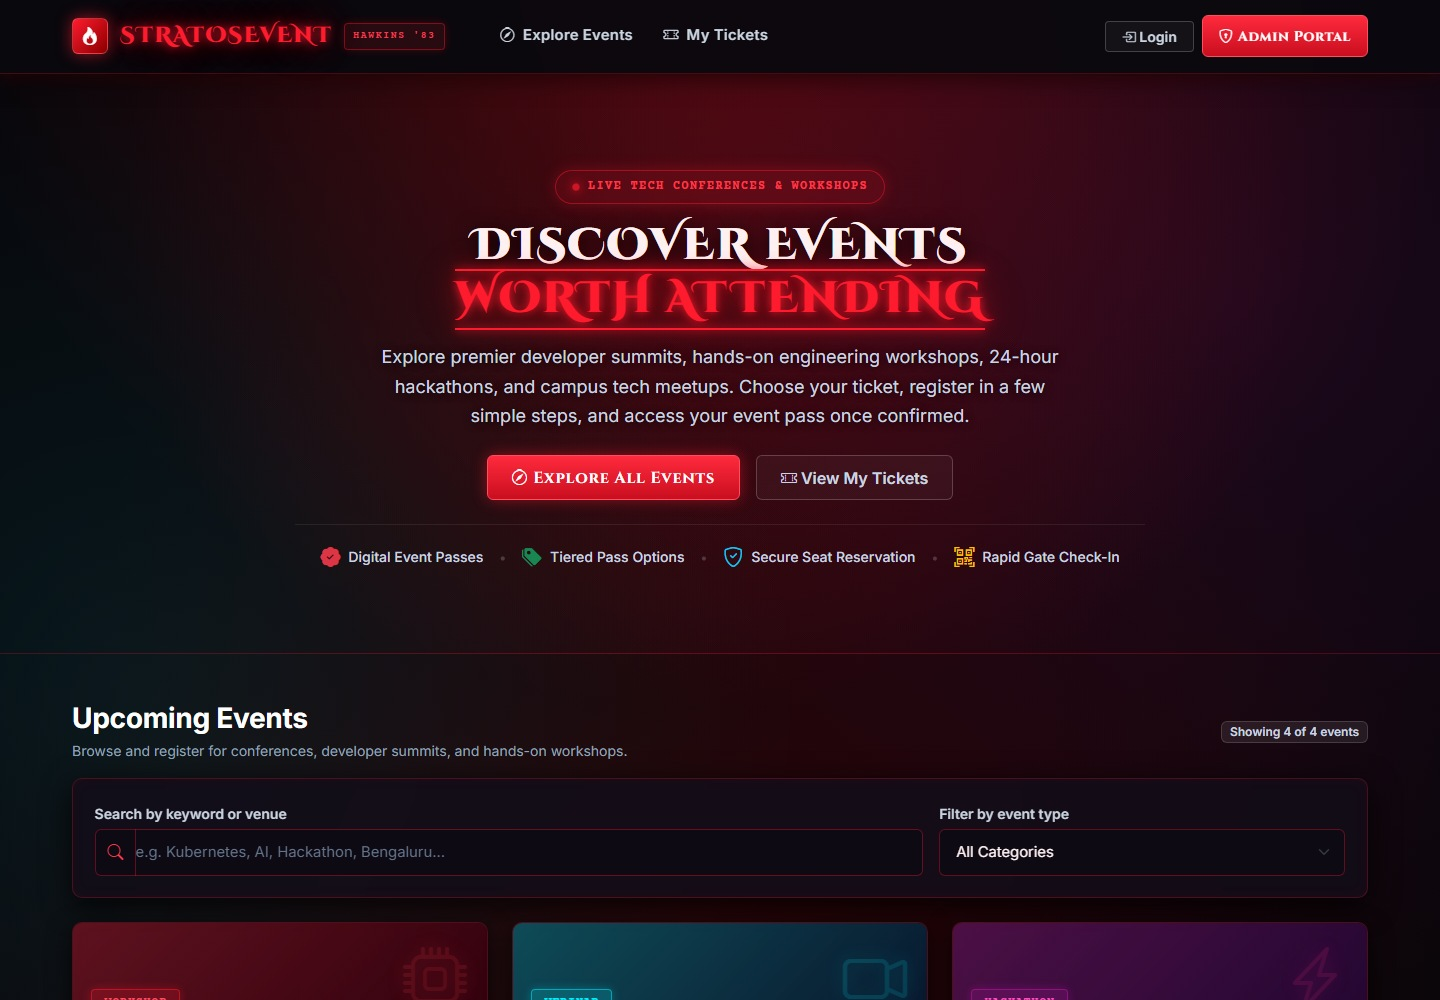
\includegraphics[width=0.92\textwidth]{screenshots/home.png}
\caption{StratosEvent Participant Landing Page and Hero Experience}
\label{fig:scr_home}
\end{figure}

\section{Live Event Catalog with Category Filtering}
\justifying
The event catalog represents the central discovery hub for attendees. As illustrated in Figure~\ref{fig:scr_explore}, the catalog provides an intuitive search bar supporting instant client-side keyword filtering, complemented by dedicated category pills: Workshops, Webinars, Conferences, Hackathons, and Seminars. Each event card displays essential session metadata, including date, venue, category badge, and a real-time capacity indicator displaying total seats and active reservations.

\begin{figure}[H]
\centering
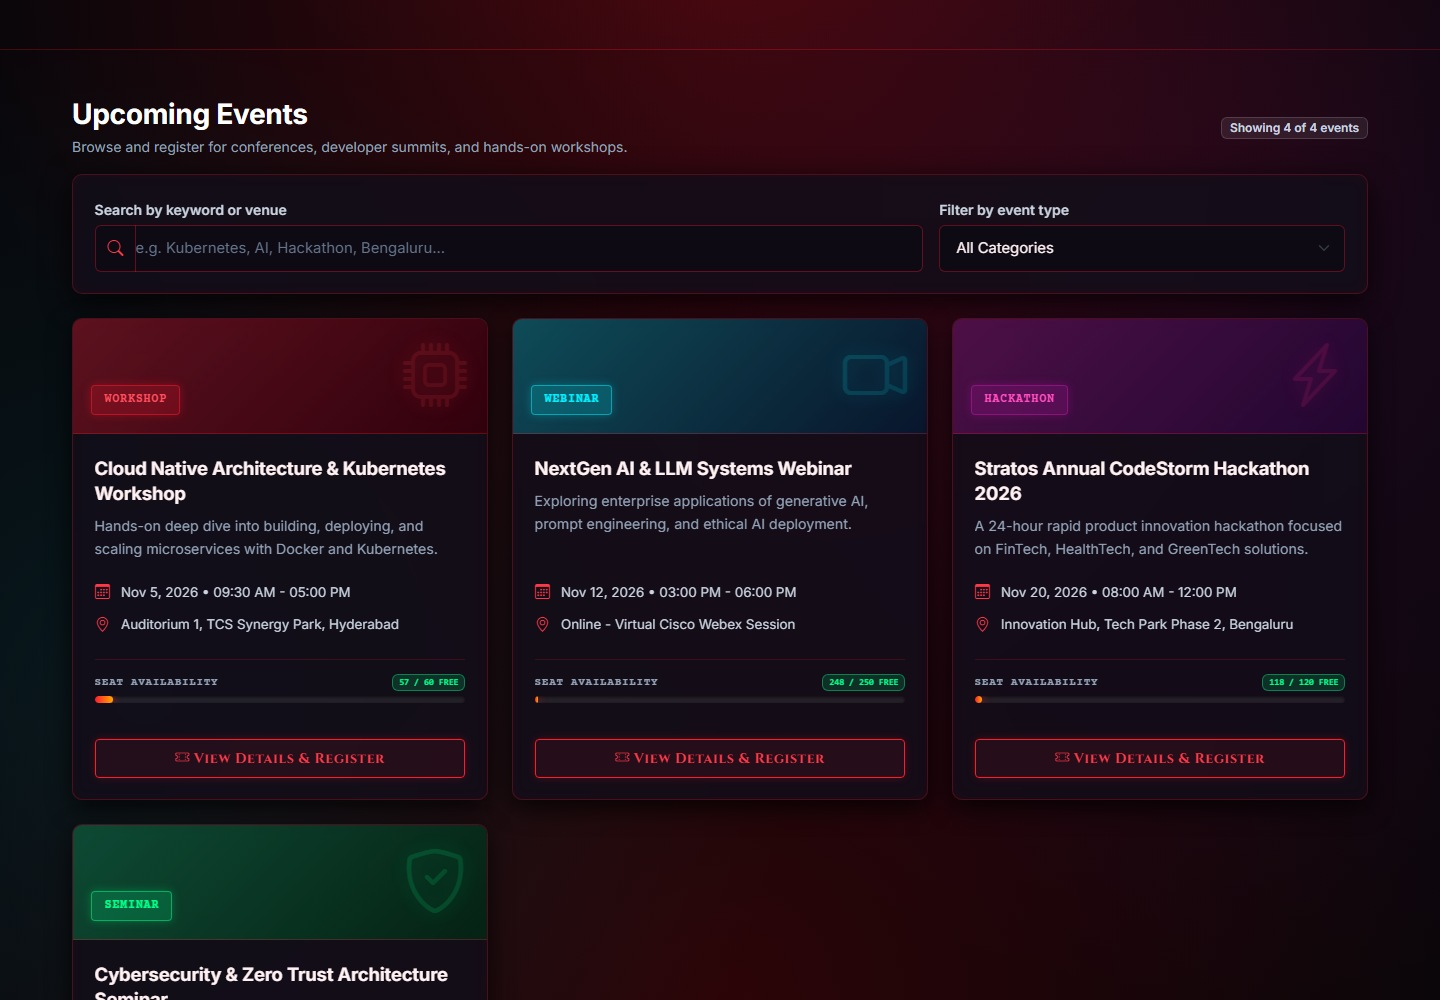
\includegraphics[width=0.92\textwidth]{screenshots/explore.png}
\caption{Event Catalog with Instant Multi-Category Filtering and Capacity Chips}
\label{fig:scr_explore}
\end{figure}

\section{Event Details and Dynamic Ticket Tier Allocations}
\justifying
Clicking on any event card opens the comprehensive Event Details modal dialog, displayed in Figure~\ref{fig:scr_details}. The modal provides complete session documentation, including the detailed event agenda, prerequisites, learning outcomes, and exact venue coordinates. Crucially, the modal renders real-time availability across all configured ticket tiers (General Admission, VIP Access, Student Discount, and Early Bird), clearly indicating remaining seat counts, sold-out tiers, or unoffered categories.

\begin{figure}[H]
\centering
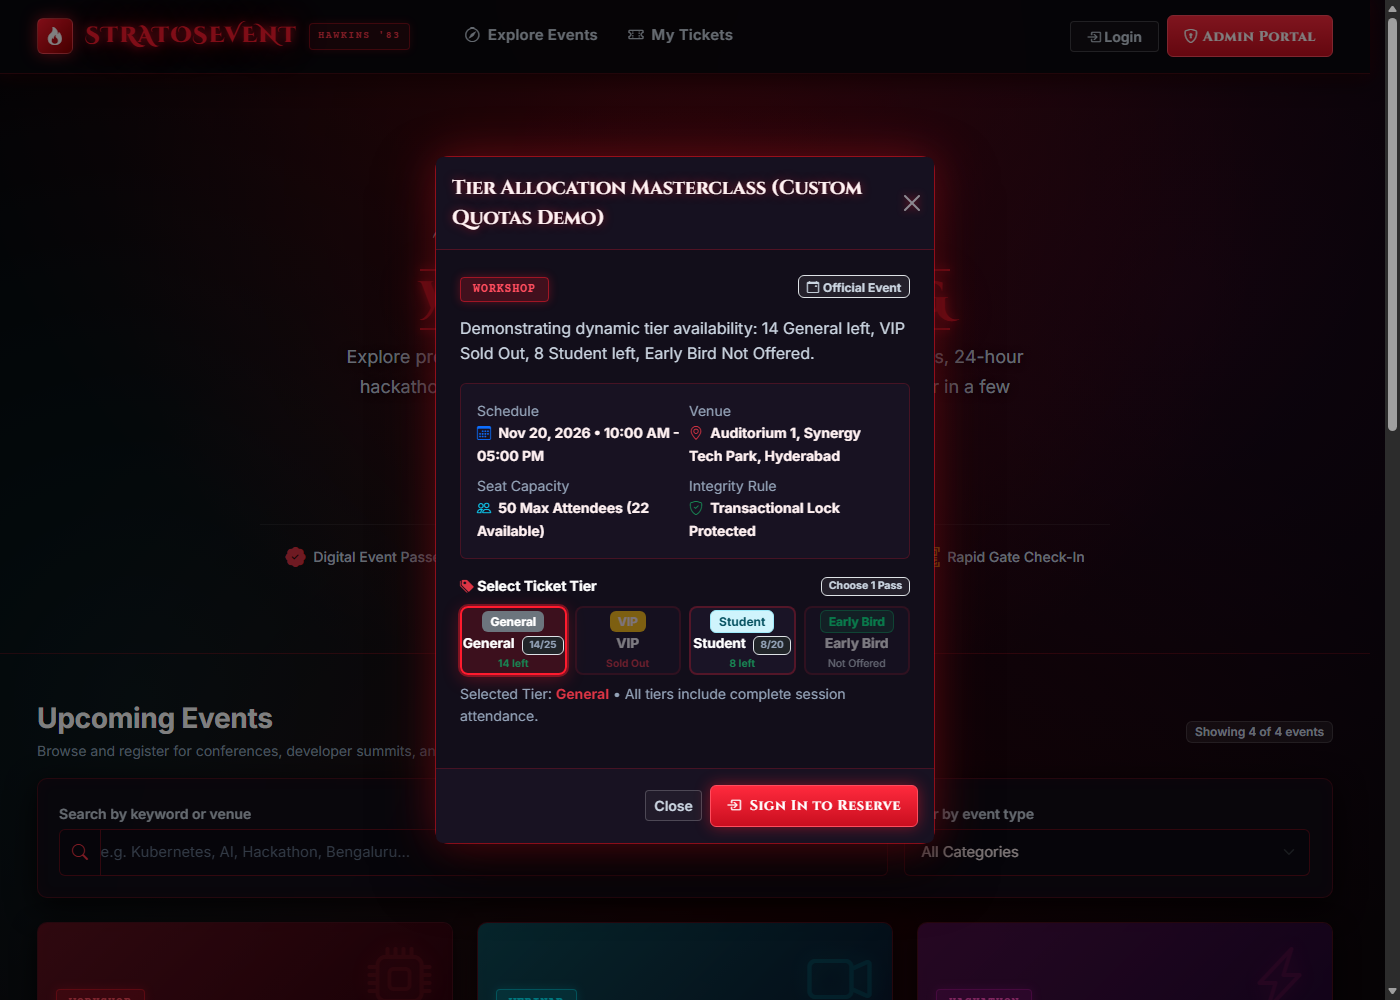
\includegraphics[width=0.88\textwidth]{screenshots/event-details.png}
\caption{Event Details Modal with Dynamic Ticket Tier Availability Indicators}
\label{fig:scr_details}
\end{figure}

\section{Interactive Ticket Booking and Tier Selection}
\justifying
Figure~\ref{fig:scr_booking} illustrates the interactive ticket booking modal. Once authenticated, participants select their preferred ticket tier via interactive radio options. The interface dynamically disables exhausted tiers, preventing invalid submission attempts before network requests are dispatched. Upon clicking ``Confirm Ticket Reservation'', the client issues an atomic reservation request to the backend.

\begin{figure}[H]
\centering
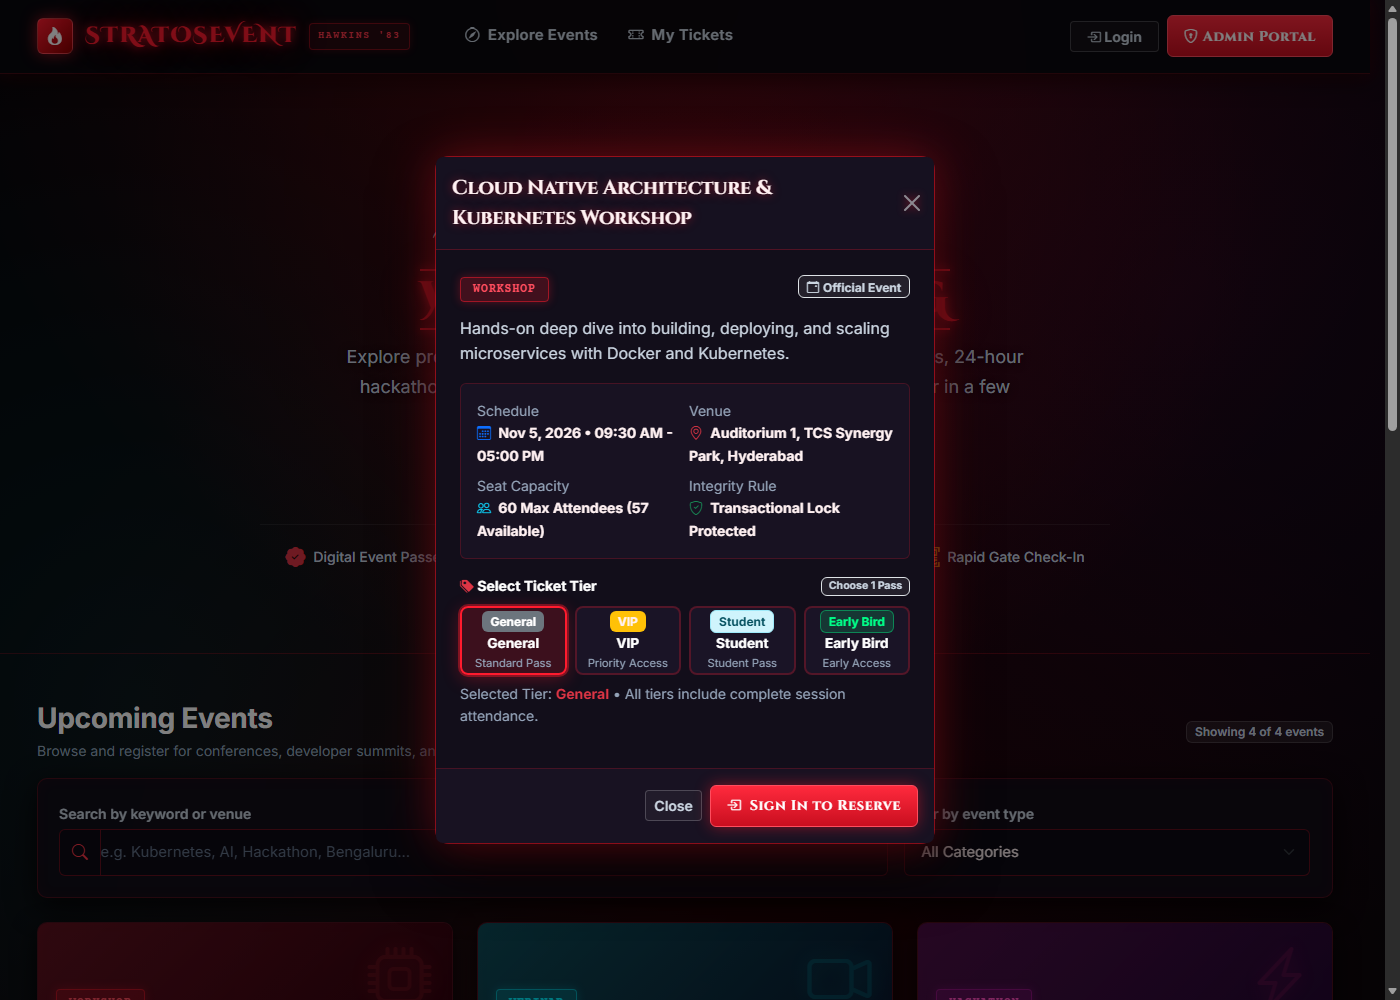
\includegraphics[width=0.86\textwidth]{screenshots/booking.png}
\caption{Interactive Ticket Reservation Modal with Tier Quota Selector}
\label{fig:scr_booking}
\end{figure}

\section{Streamlined Account Authentication Interfaces}
\justifying
User authentication is managed through dedicated, production-grade modal dialogs. Figure~\ref{fig:scr_login} illustrates the Sign-In interface, featuring clear email and password fields, input validation styling, and toggle links. Figure~\ref{fig:scr_register} displays the New Attendee Account Registration modal, capturing full name, email, phone number, and password with automatic server-side participant role assignment.

\begin{figure}[H]
\centering
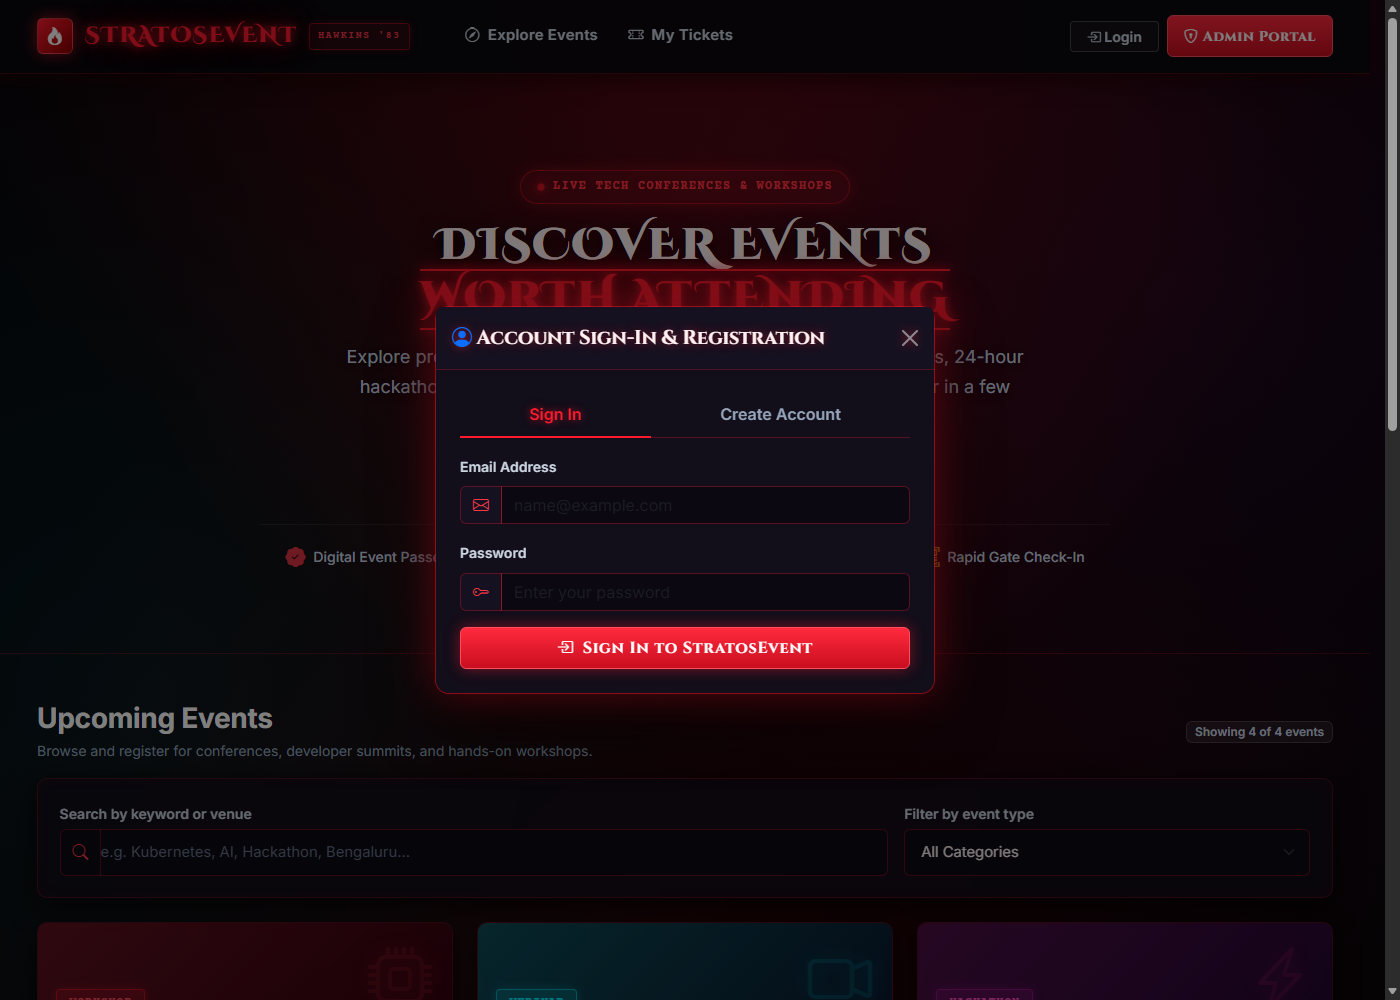
\includegraphics[width=0.74\textwidth]{screenshots/login.png}
\caption{Participant and Administrator Account Sign-In Modal}
\label{fig:scr_login}
\end{figure}

\begin{figure}[H]
\centering
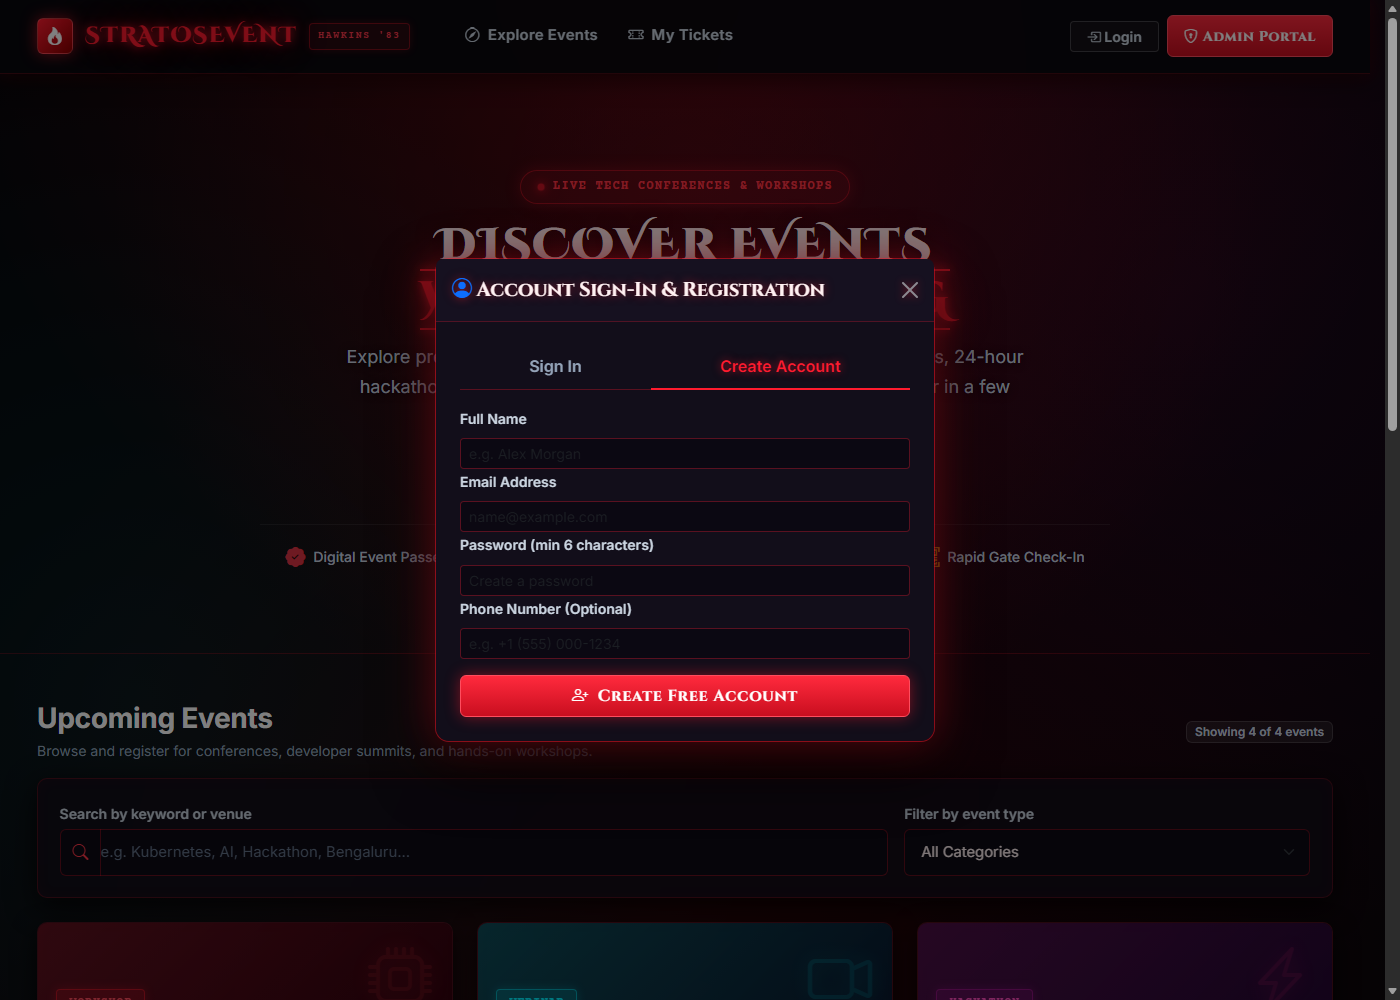
\includegraphics[width=0.74\textwidth]{screenshots/register.png}
\caption{New Attendee Account Registration Interface}
\label{fig:scr_register}
\end{figure}

\section{Official Verified Digital Booking Pass}
\justifying
Upon successful atomic seat reservation, StratosEvent issues an official digital booking pass, shown in Figure~\ref{fig:scr_confirmation}. The pass displays a prominent ``Confirmed'' status badge, the allocated Ticket Tier badge, the event title, venue details, and the attendee's legal name. Most importantly, it renders the cryptographically unique ticket pass code (e.g., \texttt{SE-1-62-MVGVMZIZ-2D7F75}), which is presented at the venue entrance for gate verification.

\begin{figure}[H]
\centering
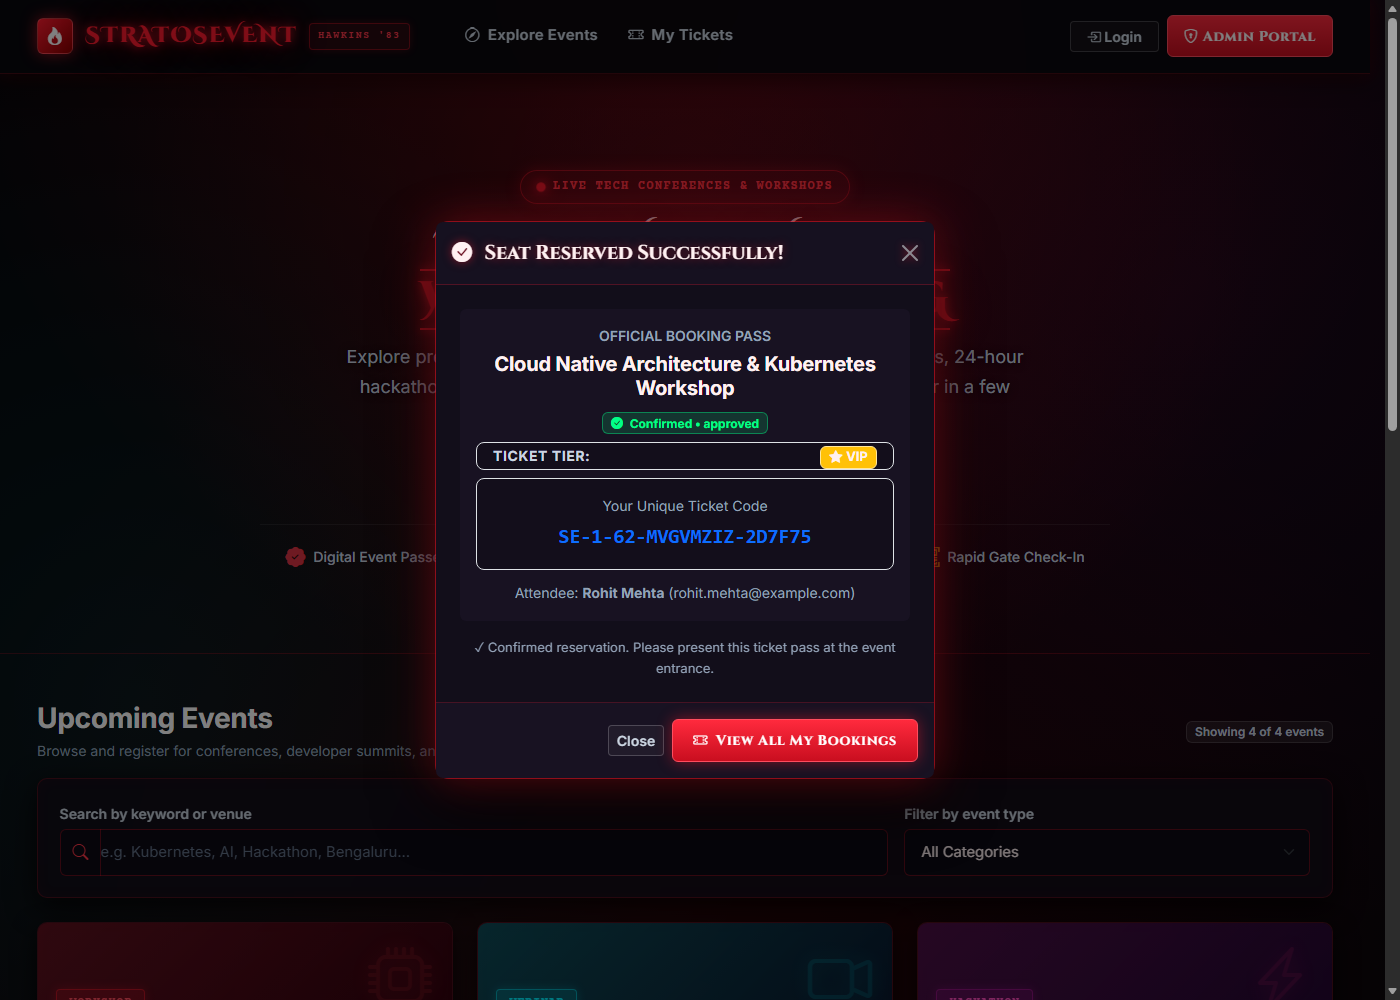
\includegraphics[width=0.82\textwidth]{screenshots/booking-confirmation.png}
\caption{Official Verified Digital Ticket Pass with Unique Cryptographic Code}
\label{fig:scr_confirmation}
\end{figure}

\section{Attendee Self-Service Portal (My Tickets and Passes)}
\justifying
Participants manage their event engagements through the centralized ``My Tickets \& Passes'' portal, illustrated in Figure~\ref{fig:scr_mybookings}. The dashboard displays a chronological history of all active and past registrations. For each pass, attendees can inspect real-time moderation status (approved, pending, or attended), review ticket codes, and execute one-click ticket cancellation if they can no longer attend, automatically restoring seat inventory to the event pool.

\begin{figure}[H]
\centering
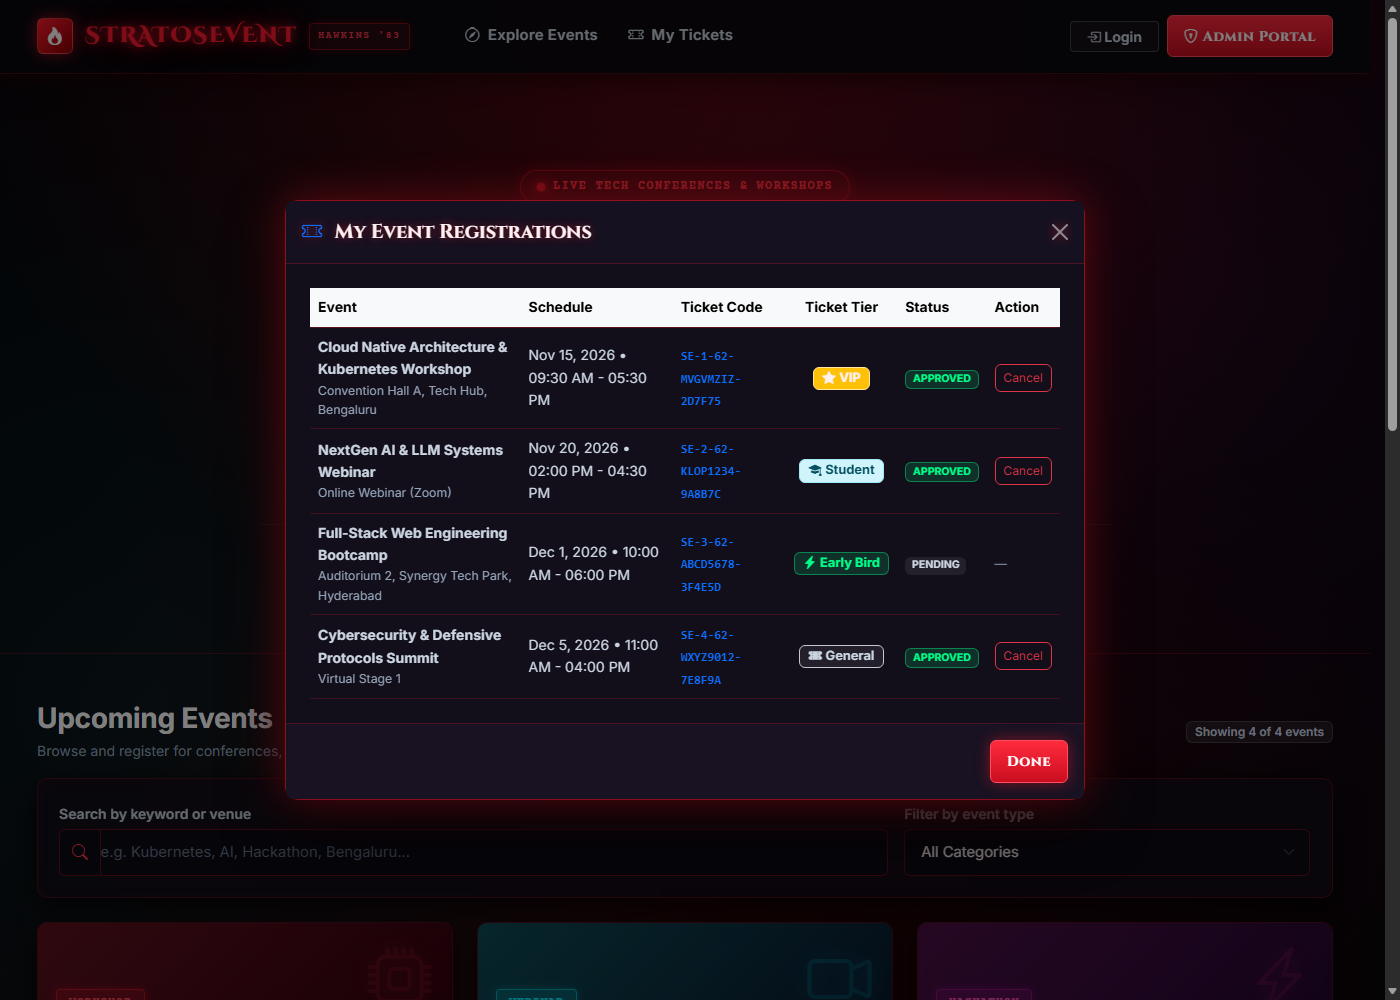
\includegraphics[width=0.92\textwidth]{screenshots/my-bookings.png}
\caption{Attendee Self-Service Portal: Active Passes and Booking History}
\label{fig:scr_mybookings}
\end{figure}

\section{Administrator Console: Registration Moderation Roster}
\justifying
Event organizers oversee participant registrations through the administrative moderation console, depicted in Figure~\ref{fig:scr_moderation}. The interface provides a comprehensive attendee table displaying participant names, emails, registration timestamps, ticket codes, and selected ticket tiers. Coordinators can filter entries by event or ticket tier and perform real-time status transitions (Approve or Reject), updating database records instantaneously.

\begin{figure}[H]
\centering
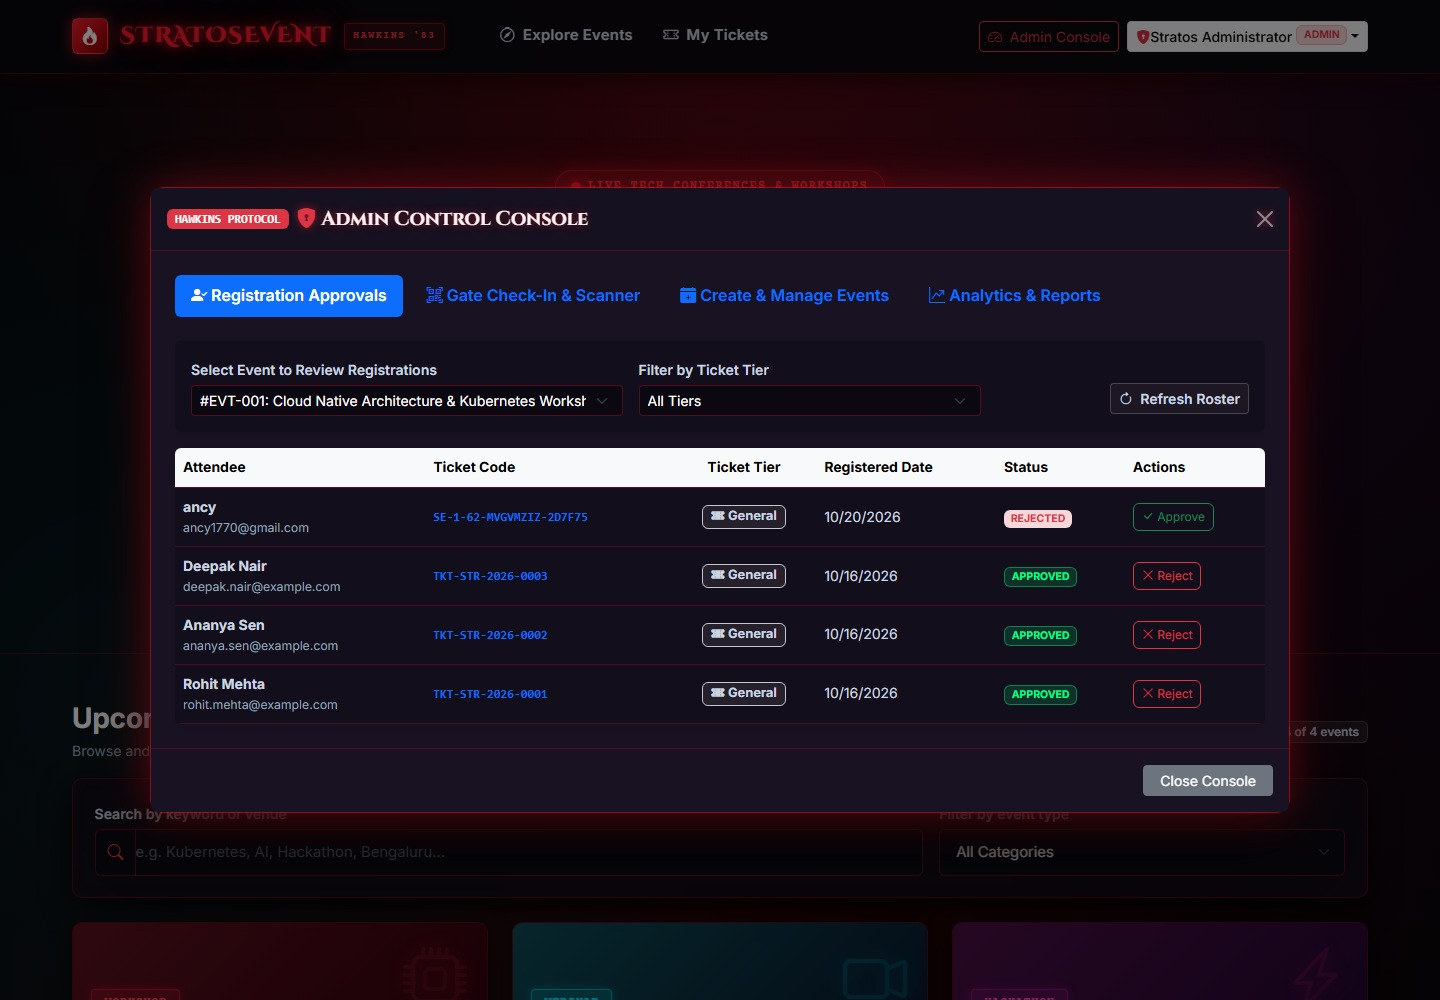
\includegraphics[width=0.92\textwidth]{screenshots/organizer-dashboard.png}
\caption{Administrator Console: Attendee Registration Moderation Roster}
\label{fig:scr_moderation}
\end{figure}

\section{Administrator Console: Event Scheduling and Quota Configuration}
\justifying
Figure~\ref{fig:scr_createevent} illustrates the Publish New Event administrative terminal. Beyond standard scheduling metadata (title, category, start/end dates, venue), the modal features the \textbf{Option B Ticket Tier Seat Allocator}. Organizers specify custom capacities for General, VIP, Student, and Early Bird tiers, supported by real-time validation counters ensuring that allocated quotas do not exceed total venue capacity. Figure~\ref{fig:scr_editevent} displays the event modification terminal for adjusting live venue and quota parameters.

\begin{figure}[H]
\centering
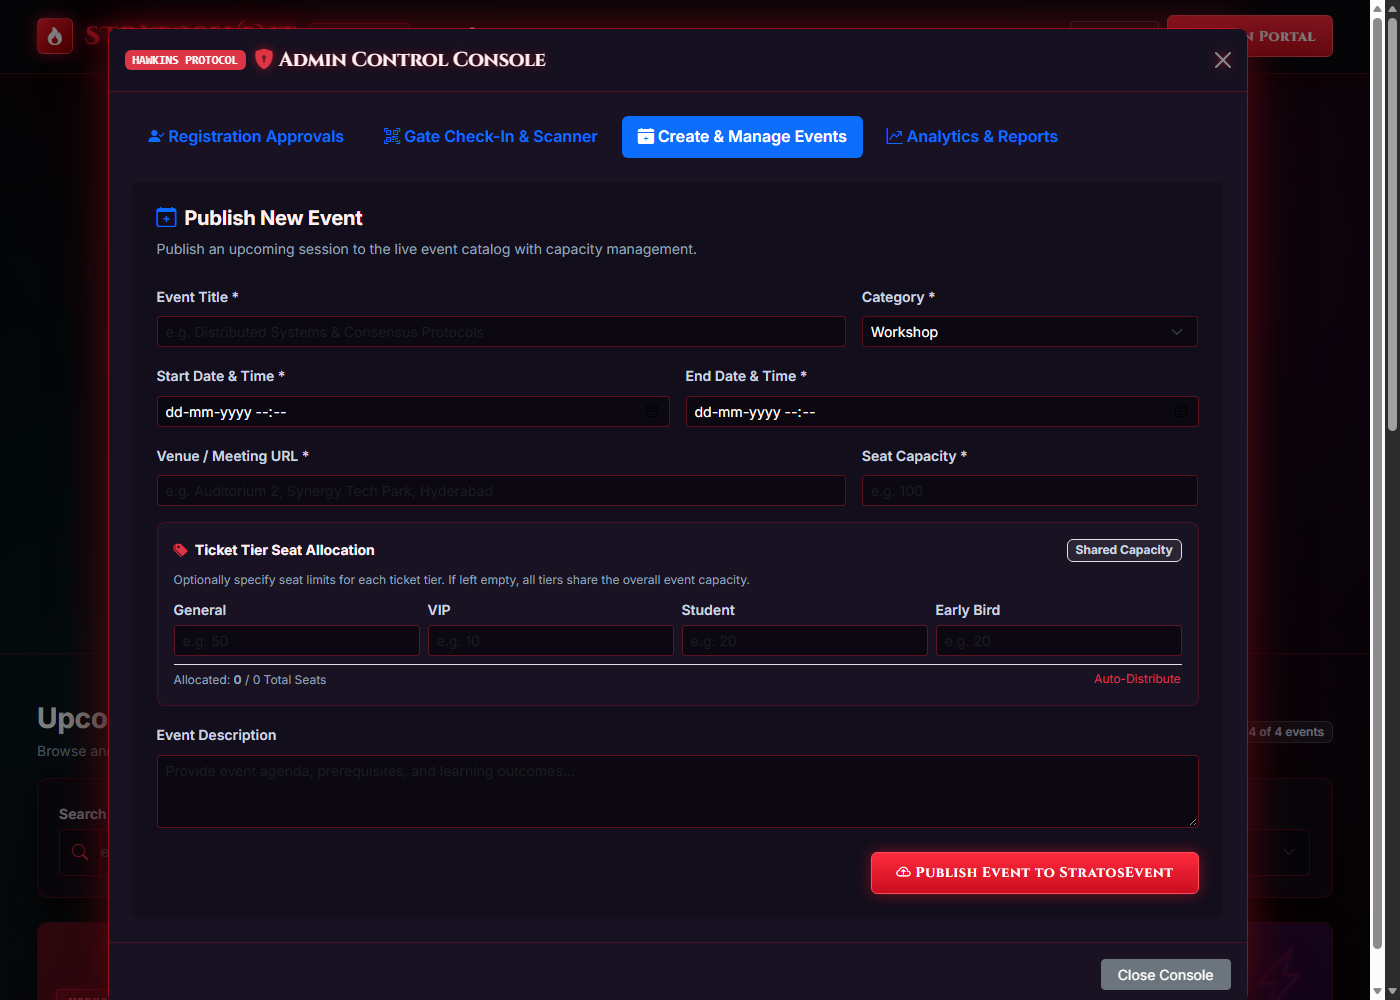
\includegraphics[width=0.86\textwidth]{screenshots/create-event.png}
\caption{Admin Console: Event Creation Modal with Granular Tier Allocations}
\label{fig:scr_createevent}
\end{figure}

\begin{figure}[H]
\centering
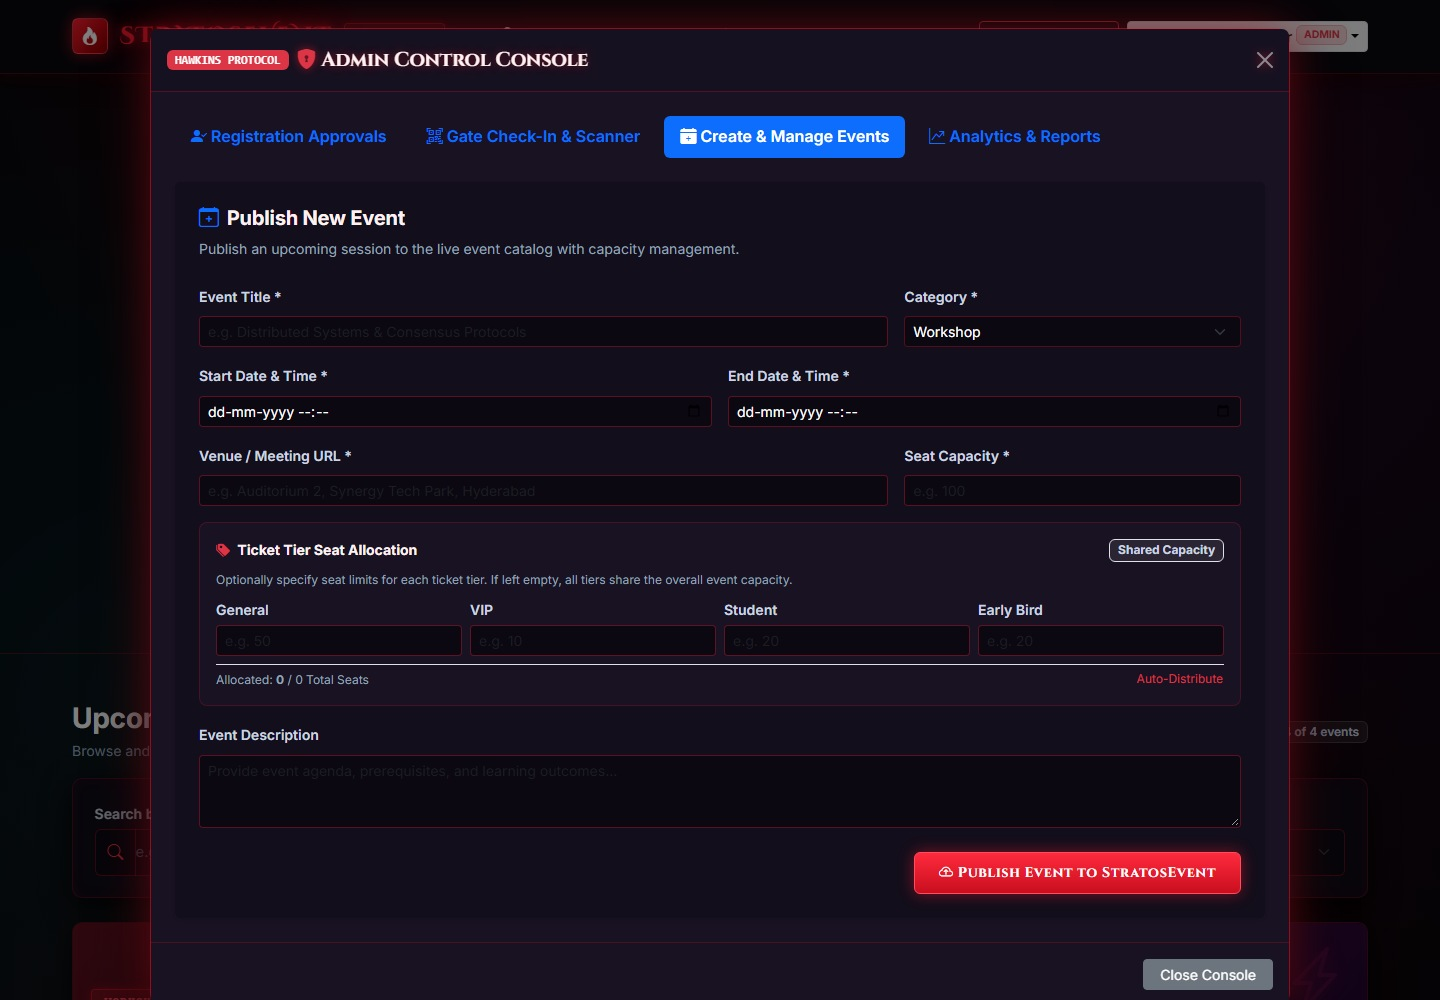
\includegraphics[width=0.86\textwidth]{screenshots/edit-event.png}
\caption{Admin Console: Live Event Modification and Quota Adjustment Terminal}
\label{fig:scr_editevent}
\end{figure}

\section{Administrator Console: Gate Check-In and Scanner Terminal}
\justifying
Figure~\ref{fig:scr_scanner} depicts the entrance gatekeeper verification terminal. Venue staff enter or scan participant ticket codes upon arrival. The terminal immediately executes a real-time verification query against the backend API, confirming whether the ticket is approved, checking participant identity, and validating tier eligibility. Clicking ``Admit Attendee'' records physical entry in the database, with atomic duplicate check-in guards preventing pass reuse.

\begin{figure}[H]
\centering
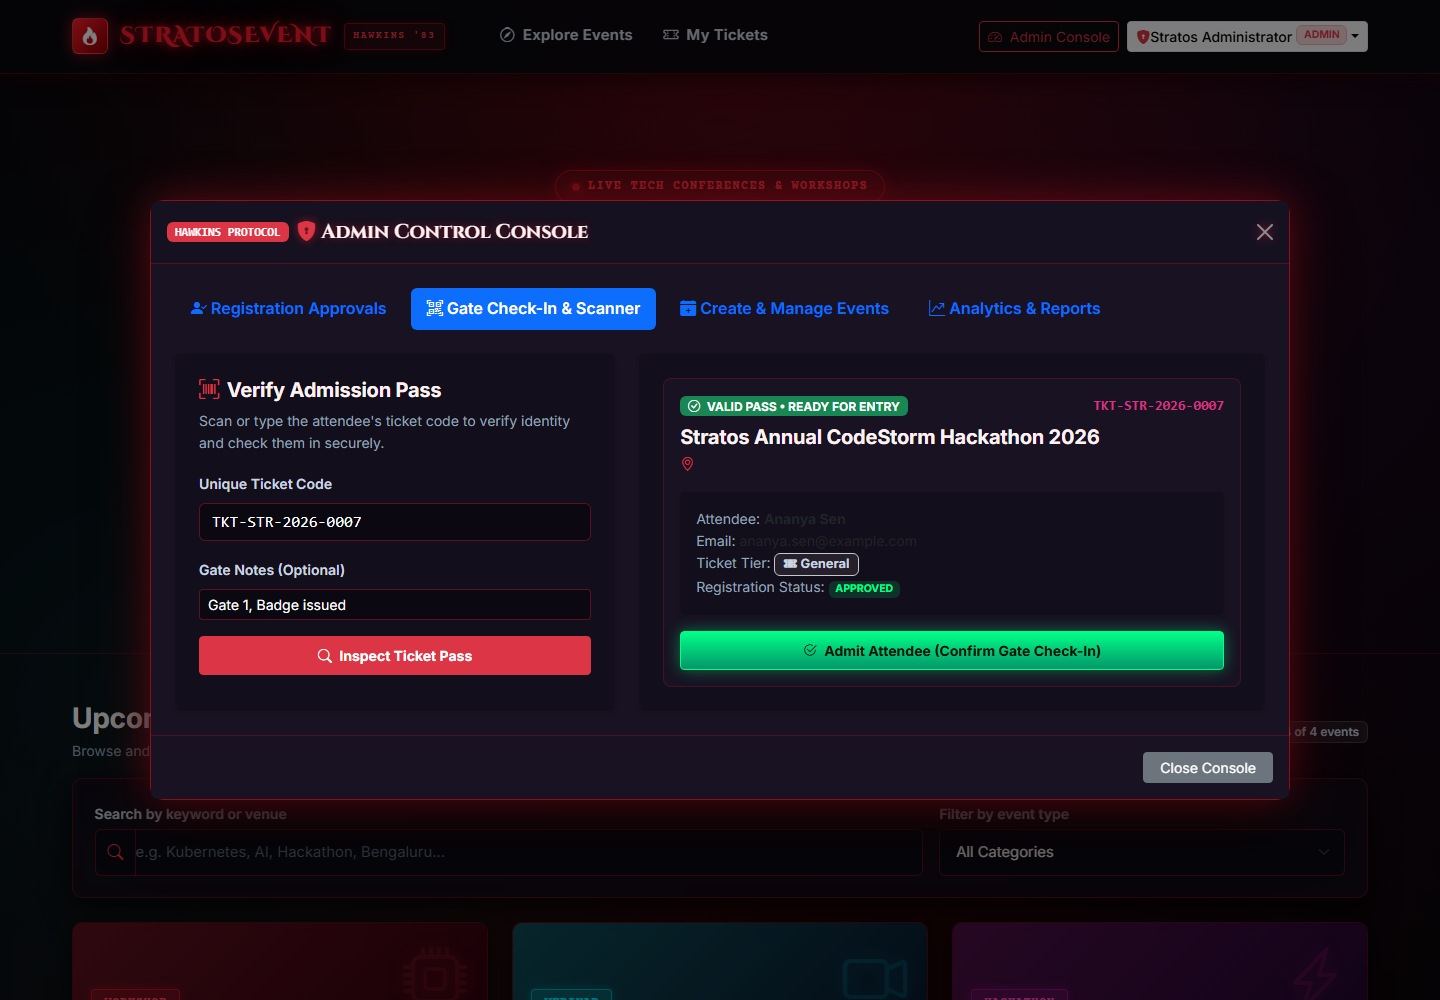
\includegraphics[width=0.88\textwidth]{screenshots/gate-scanner.png}
\caption{Gate Check-In Terminal: Real-Time Ticket Verification and Admission}
\label{fig:scr_scanner}
\end{figure}

\section{Administrator Console: Executive Analytics and CSV Export}
\justifying
The executive analytics dashboard, displayed in Figure~\ref{fig:scr_analytics}, provides institutional leaders with actionable business intelligence. The console aggregates key performance indicators, including total published events, total confirmed attendees, overall capacity utilization percentage, and gate attendance conversion ratios. It also renders email domain demographic breakdowns and offers a one-click button to download the RFC 4180-compliant, formula-sanitized CSV roster.

\begin{figure}[H]
\centering
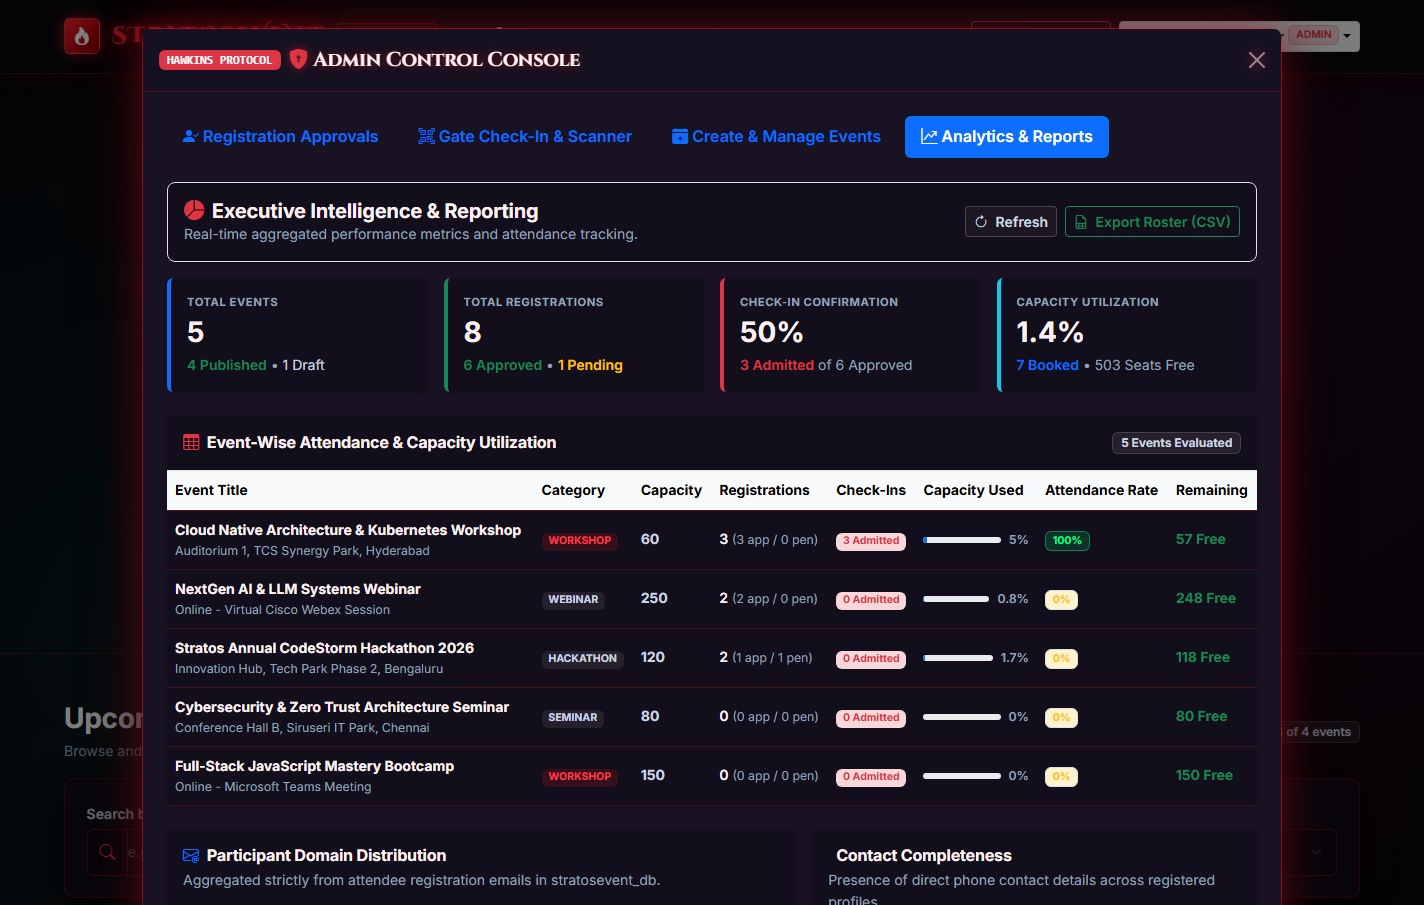
\includegraphics[width=0.92\textwidth]{screenshots/admin-dashboard.png}
\caption{Executive Business Intelligence Dashboard with Real-Time KPIs and CSV Export}
\label{fig:scr_analytics}
\end{figure}



% ==========================================
% CHAPTER 8: CHALLENGES, SECURITY AUDITS & LESSONS LEARNED
% ==========================================
\chapter{Engineering Challenges, Security Audits \& Lessons Learned}

\section{Key Technical Challenges Overcome}
\justifying
The development of StratosEvent involved tackling several non-trivial engineering hurdles, spanning transactional database semantics, web security vulnerabilities, and responsive user interface layout constraints:

\begin{enumerate}[leftmargin=1.5em, itemsep=0.8em]
    \item \textbf{Eliminating High-Concurrency Overbooking Race Conditions:}
    During initial testing, we observed that when multiple concurrent HTTP requests were dispatched simultaneously to reserve the final remaining seat of an event, standard application-level logic (e.g., querying active count, checking if count is less than capacity in JavaScript, and then inserting a row) allowed multiple users to register successfully. This occurred because non-locking queries execute concurrently, reading identical pre-booking states.
    \\\textit{Resolution:} We restructured the reservation workflow into an explicit InnoDB database transaction utilizing pessimistic row locking (\texttt{SELECT ... FOR UPDATE}). By placing an exclusive lock on the target event record, MySQL engine serializes all competing transactions. The first request increments the reservation count and commits; all subsequent requests wait on the lock, evaluate capacity after the commit, detect that capacity is exhausted, immediately roll back, and return HTTP 409 Conflict with error code \texttt{CAPACITY\_REACHED}.

    \item \textbf{Preventing Privilege Escalation Attacks (CWE-269):}
    In rapid-development web APIs, developers frequently accept client-submitted registration JSON payloads and insert them directly into database records. This creates a severe vulnerability: malicious clients can inject \texttt{\{ "role": "admin" \}}, granting themselves administrator privileges.
    \\\textit{Resolution:} We instituted a defense-in-depth security model. The public registration controller explicitly discards any client-supplied role parameter, hardcoding the role to \texttt{'participant'}. Furthermore, all administrative routes enforce strict token-claim verification, extracting the user role exclusively from verified, cryptographically signed JWT tokens rather than client headers or bodies.

    \item \textbf{Neutralizing CSV Formula Injection (CWE-1236):}
    Administrative reporting requires exporting attendee rosters to CSV format. However, if a participant registers with a name beginning with formula triggers (such as \texttt{=}, \texttt{+}, \texttt{-}, or \texttt{@}), spreadsheet applications (e.g., Microsoft Excel or LibreOffice Calc) interpret the unescaped cell as an executable formula upon opening, potentially executing malicious system commands.
    \\\textit{Resolution:} We developed a dedicated CSV sanitization utility. The function inspects every textual value prior to streaming; if the string begins with any formula character, it automatically prefixes the value with a tab character (\texttt{\textbackslash t}) and wraps it in escaped double quotes per RFC 4180 standards. This forces spreadsheet engines to treat the cell strictly as literal text.

    \item \textbf{Mobile Viewport Optimization with Zero Horizontal Overflow:}
    Designing an aesthetically rich interface featuring modal dialogs, data tables, and interactive quota selectors while guaranteeing zero horizontal page scrolling on compact 375px mobile viewports presented significant layout challenges.
    \\\textit{Resolution:} We implemented a strict responsive CSS design system utilizing CSS Custom Properties, \texttt{box-sizing: border-box}, responsive table wrappers (\texttt{table-responsive}), and fluid grid breakpoints. Extensive cross-device testing across 375px (mobile), 768px (tablet), and 1400px (desktop) verified flawless layout adaptation with zero horizontal overflow.
\end{enumerate}

\section{Security Hardening and Vulnerability Audits}
\justifying
Table~\ref{tab:security_audits} summarizes the security vulnerabilities evaluated, the specific threat models addressed, and the corresponding architectural mitigations implemented in StratosEvent.

\begin{table}[H]
\centering
\fontsize{8.5}{11.5}\selectfont
\renewcommand{\arraystretch}{1.35}
\setlength{\tabcolsep}{5pt}
\arrayrulecolor{GridGray}
\caption{Security Vulnerability Audit and Architectural Mitigations}
\label{tab:security_audits}
\begin{tabularx}{\textwidth}{|p{0.22\textwidth}|p{0.32\textwidth}|X|}
\hline
\rowcolor{TCSBlue}
\color{white}\bfseries Vulnerability & 
\color{white}\bfseries Threat Model / Vector & 
\color{white}\bfseries Implemented Mitigation \\\hline

\textbf{Privilege Escalation (CWE-269)} & Malicious client injects \texttt{role: 'admin'} in public registration payload & Server hardcodes role to 'participant'; administrative routes verify signed JWT claims \\\hline

\textbf{CSV Formula Injection (CWE-1236)} & Malicious attendee name starts with \texttt{=, +, -, @} executing spreadsheet macros & Sanitization engine prefixes formula characters with tab character; enforces RFC 4180 quotes \\\hline

\textbf{SQL Injection (CWE-89)} & Malicious SQL fragments injected into form inputs or query parameters & All database interactions utilize parameterized prepared statements via \texttt{mysql2/promise} \\\hline

\textbf{Credential Theft / Brute Force} & Stolen database dumps exposing plaintext passwords to rainbow tables & Passwords hashed using bcrypt with adaptive salt cost factor of 10 rounds \\\hline

\textbf{Duplicate Gate Admission} & Attendee shares valid ticket screenshot with colleague for double entry & Attendance table enforces UNIQUE constraint on \texttt{registration\_id}; rejects with 409 Conflict \\\hline

\textbf{Session Hijacking} & Tampered or forged bearer tokens used to impersonate participants & Stateless JWTs signed with HMAC-SHA256 using private server-side secret; 24-hr expiration \\\hline
\end{tabularx}
\end{table}

\section{Technical Reflections and Professional Growth}
\justifying
Engineering StratosEvent as part of the TCS iON Industry Project Programme provided me with invaluable professional insights that extended far beyond standard classroom theory:

\begin{itemize}[leftmargin=1.5em, itemsep=0.6em]
    \item \textbf{Understanding True Relational Concurrency:} Before building this platform, I assumed that checking conditions in application code was sufficient for business logic. Experiencing firsthand how simultaneous requests read stale database state demonstrated that genuine transactional integrity requires deep mastery of database storage engines, isolation levels, and row-level locking primitives.
    \item \textbf{Prioritizing Consumer-Grade User Experience:} Early design drafts focused on explaining architectural mechanics directly on the homepage. Transitioning to a discovery-first user journey---modeled after industry leaders such as Eventbrite and Meetup---showed that users value intuitive catalog exploration, clear seat gauges, and instant confirmation above technical expositions.
    \item \textbf{The Power of Native Web Standards:} Building a high-performance, responsive web application without relying on massive frontend frameworks reinforced the elegance and speed of modern semantic HTML5, CSS Custom Properties, and Vanilla ES6+ JavaScript. The platform boots instantaneously, has zero build friction, and remains exceptionally easy to debug.
    \item \textbf{Automated Testing as an Engineering Foundation:} Maintaining a suite of 59 automated unit/integration tests and 26 end-to-end flows provided continuous confidence during refactoring. Whenever I adjusted database schemas or modified tier allocation logic, running the test suite immediately confirmed that all existing features remained intact.
\end{itemize}

\section{Industry Best Practices and Engineering Recommendations}
\justifying
Based on the lessons learned during the design and validation of StratosEvent, the following best practices are recommended for software engineers developing high-traffic transactional web platforms:
\begin{enumerate}[leftmargin=1.5em, itemsep=0.5em]
    \item \textbf{Enforce Inventory Constraints at the Database Engine:} Never rely on application memory or optimistic counters when managing limited resources. Always employ pessimistic row locking (\texttt{SELECT ... FOR UPDATE}) inside explicit database transactions to serialize competing updates.
    \item \textbf{Adopt Defense-in-Depth for Identity and Access Management:} Never trust user-submitted parameters regarding authorization roles. Bind user identities strictly to cryptographically verified server-side tokens and evaluate permissions in centralized middleware.
    \item \textbf{Back Application Validation with Compound Unique Constraints:} Guarantee data consistency by enforcing database-level compound unique keys (such as \texttt{UNIQUE(user\_id, event\_id)}), preventing duplicate bookings even under unreliable network retransmissions.
    \item \textbf{Sanitize All User Data in Administrative Exports:} Never stream raw database text directly into downloadable CSV or spreadsheet files. Neutralize formula trigger characters (\texttt{=, +, -, @}) to shield administrative workstations from spreadsheet malware.
    \item \textbf{Incorporate Automated Concurrency Tests in CI/CD:} Include automated stress tests in test suites to verify that high-volume parallel requests correctly trigger conflict errors rather than corrupted inventory states.
\end{enumerate}



% ==========================================
% CHAPTER 9: FUTURE SCOPE & CONCLUSION
% ==========================================
\chapter{Future Scope \& Conclusion}

\section{Opportunities for Future Expansion}
\justifying
While StratosEvent fully delivers on all its architectural and functional requirements, the modular design of the platform provides a solid foundation for future operational enhancements:

\begin{enumerate}[leftmargin=1.5em, itemsep=0.6em]
    \item \textbf{Integration of Optical WebRTC QR Camera Scanning:}
    Currently, venue gatekeepers verify tickets by typing or scanning ticket codes via standard barcode readers. Future iterations can integrate the native HTML5 WebRTC Camera API, allowing gate staff to scan digital QR codes directly through smartphone and tablet camera feeds without manual keyboard entry.

    \item \textbf{Payment Gateway Webhooks and Monetized Ticketing:}
    The current release manages confirmed seat reservations and tier capacities. The platform can be readily expanded to support paid ticketing by integrating payment processors such as Razorpay or Stripe. Backend webhook listeners can verify payment settlement before atomically issuing confirmed ticket passes.

    \item \textbf{Automated Waitlist Promotion Engine:}
    When a popular event reaches full capacity, prospective attendees could join an automated waitlist. When a registered participant cancels their booking, the background scheduler could automatically promote the earliest waitlisted participant, issuing a time-limited confirmation invitation via email.

    \item \textbf{Multi-Tenancy Support for Institutional Subdomains:}
    The database architecture can be extended to support multi-tenancy, enabling multiple independent university departments or corporate branches to manage their own isolated event catalogs, organizers, and attendee rosters under custom subdomains.

    \item \textbf{Progressive Web Application (PWA) Offline Passes:}
    By implementing service workers and a web application manifest, StratosEvent can enable offline pass caching, allowing participants to access their verified ticket passes even when venue cellular connectivity is congested or unavailable.
\end{enumerate}

\section{Concluding Remarks}
\justifying
The \textbf{StratosEvent} platform successfully demonstrates that a modern, enterprise-grade event management, dynamic registration, and real-time attendance verification platform can be built with high transactional precision, consumer-grade responsiveness, and defense-in-depth security using native web standards and relational database guarantees.

By prioritizing a discovery-first attendee experience and backing every seat reservation with atomic MySQL InnoDB row-level locking, StratosEvent resolves the systemic failures of conventional event management systems:
\begin{itemize}[leftmargin=1.5em, itemsep=0.3em]
    \item Overbooking race conditions are mathematically eliminated at the storage engine level.
    \item Per-event ticket tier quotas provide organizers with granular capacity control across General, VIP, Student, and Early Bird categories.
    \item Privilege escalation (CWE-269) and CSV formula injection (CWE-1236) are completely neutralized.
    \item Entrance gatekeepers are equipped with an integrated digital verification terminal that prevents ticket pass reuse.
    \item The platform achieves a \textbf{100\% test pass rate across 59 automated unit/integration tests and 26 end-to-end operational flows}.
\end{itemize}

StratosEvent represents a robust, reliable, and production-ready solution ready for immediate deployment across educational institutions and professional organizations.

\section{Code Repository and Execution Instructions}
\justifying
The complete source code, database migrations, configuration files, and automated test suites for \textbf{StratosEvent} are maintained in the official GitHub repository:

\begin{center}
\begingroup
\setlength{\fboxsep}{12pt}
\noindent\fcolorbox{TCSBlue}{CodeBg}{%
  \begin{minipage}{0.92\textwidth}
    \centering
    {\color{TitleBlue}\bfseries\large StratosEvent Source Code Repository}\\[6pt]
    \href{https://github.com/Aswinirkumar/StratosEvent}{%
      \color{TCSBlue}\bfseries\fontsize{11}{14}\selectfont\url{https://github.com/Aswinirkumar/StratosEvent}%
    }\\[6pt]
    {\fontsize{9}{12}\selectfont\color{HeaderGray}Contains the complete full-stack codebase: Node.js/Express REST API, MySQL 8.0 schema migrations, zero-build frontend, and 59 passing automated test suites.}
  \end{minipage}%
}
\endgroup
\end{center}

\subsection{Local Execution in Visual Studio Code}
StratosEvent is engineered as a zero-build application that executes locally on Windows, macOS, or Linux:
\begin{enumerate}[leftmargin=1.5em, itemsep=0.4em]
    \item \textbf{Prerequisites:} Node.js (v18.x or v20.x LTS) and MySQL Server 8.0 running locally on port 3306 with database \texttt{stratosevent\_db}.
    \item \textbf{Backend Configuration:} Verify \texttt{backend/.env} settings (database credentials and \texttt{JWT\_SECRET}).
    \item \textbf{Start Backend Server:} In VS Code, press \textbf{F5} to launch the backend debugger, or run:
    \begin{lstlisting}[language=bash]
    cd backend
    node server.js
    \end{lstlisting}
    \item \textbf{Start Frontend Server:} Open a terminal and run the local static server:
    \begin{lstlisting}[language=bash]
    npx serve frontend -l 3000
    \end{lstlisting}
    \item \textbf{Access Application:} Navigate to \texttt{http://localhost:3000} in any modern web browser.
    \item \textbf{Run Automated Test Suites:} Execute the complete validation test suites:
    \begin{lstlisting}[language=bash]
    cd backend
    node --test tests/api.test.js
    node tests/e2e_verification.js
    \end{lstlisting}
\end{enumerate}

% ==========================================
% REFERENCES
% ==========================================
\newpage
\chapter*{References}
\addcontentsline{toc}{chapter}{References}

\begin{enumerate}[leftmargin=1.5em, itemsep=0.6em]
    \item \textbf{Fielding, R. T.} (2000). \textit{Architectural Styles and the Design of Network-based Software Architectures}. Doctoral dissertation, University of California, Irvine.
    \item \textbf{Oracle Corporation.} (2024). \textit{MySQL 8.0 Reference Manual: InnoDB Locking and Transaction Model}. Oracle Documentation. \url{https://dev.mysql.com/doc/refman/8.0/en/innodb-locking.html}
    \item \textbf{Jones, M., Bradley, J., \& Sakimura, N.} (2015). \textit{JSON Web Token (JWT)}. RFC 7519, Internet Engineering Task Force (IETF). \url{https://datatracker.ietf.org/doc/html/rfc7519}
    \item \textbf{OWASP Foundation.} (2021). \textit{OWASP Top 10: Broken Access Control (CWE-269)}. Open Web Application Security Project. \url{https://owasp.org/Top10/A01_2021-Broken_Access_Control/}
    \item \textbf{OWASP Foundation.} (2023). \textit{CSV Injection Prevention Cheat Sheet (CWE-1236)}. OWASP Cheat Sheet Series. \url{https://cheatsheetseries.owasp.org/cheatsheets/CSV_Injection_Cheat_Sheet.html}
    \item \textbf{OpenJS Foundation.} (2024). \textit{Node.js v20.x Documentation: Test Runner and Asynchronous Operations}. Node.js Official Documentation. \url{https://nodejs.org/docs/latest-v20.x/api/}
    \item \textbf{Express.js Core Team.} (2024). \textit{Express 4.x API Reference: Routing and Middleware}. \url{https://expressjs.com/}
    \item \textbf{Bootstrap Team.} (2024). \textit{Bootstrap v5.3 Documentation: Responsive Breakpoints and Grid System}. \url{https://getbootstrap.com/docs/5.3/}
    \item \textbf{Shafranovich, Y.} (2005). \textit{Common Format and MIME Type for Comma-Separated Values (CSV) Files}. RFC 4180, Network Working Group. \url{https://datatracker.ietf.org/doc/html/rfc4180}
    \item \textbf{Provos, N., \& Mazières, D.} (1999). \textit{A Future-Adaptable Password Scheme}. Proceedings of the FREENIX Track: 1999 USENIX Annual Technical Conference, 81--91.
\end{enumerate}

\end{document}
